% Options for packages loaded elsewhere
\PassOptionsToPackage{unicode}{hyperref}
\PassOptionsToPackage{hyphens}{url}
%
\documentclass[
]{article}
\title{AFCm}
\author{YALAOUI Akli \& BOULAOUAD ADEL}
\date{1/26/2022}

\usepackage{amsmath,amssymb}
\usepackage{lmodern}
\usepackage{iftex}
\ifPDFTeX
  \usepackage[T1]{fontenc}
  \usepackage[utf8]{inputenc}
  \usepackage{textcomp} % provide euro and other symbols
\else % if luatex or xetex
  \usepackage{unicode-math}
  \defaultfontfeatures{Scale=MatchLowercase}
  \defaultfontfeatures[\rmfamily]{Ligatures=TeX,Scale=1}
\fi
% Use upquote if available, for straight quotes in verbatim environments
\IfFileExists{upquote.sty}{\usepackage{upquote}}{}
\IfFileExists{microtype.sty}{% use microtype if available
  \usepackage[]{microtype}
  \UseMicrotypeSet[protrusion]{basicmath} % disable protrusion for tt fonts
}{}
\makeatletter
\@ifundefined{KOMAClassName}{% if non-KOMA class
  \IfFileExists{parskip.sty}{%
    \usepackage{parskip}
  }{% else
    \setlength{\parindent}{0pt}
    \setlength{\parskip}{6pt plus 2pt minus 1pt}}
}{% if KOMA class
  \KOMAoptions{parskip=half}}
\makeatother
\usepackage{xcolor}
\IfFileExists{xurl.sty}{\usepackage{xurl}}{} % add URL line breaks if available
\IfFileExists{bookmark.sty}{\usepackage{bookmark}}{\usepackage{hyperref}}
\hypersetup{
  pdftitle={AFCm},
  pdfauthor={YALAOUI Akli \& BOULAOUAD ADEL},
  hidelinks,
  pdfcreator={LaTeX via pandoc}}
\urlstyle{same} % disable monospaced font for URLs
\usepackage[margin=1in]{geometry}
\usepackage{color}
\usepackage{fancyvrb}
\newcommand{\VerbBar}{|}
\newcommand{\VERB}{\Verb[commandchars=\\\{\}]}
\DefineVerbatimEnvironment{Highlighting}{Verbatim}{commandchars=\\\{\}}
% Add ',fontsize=\small' for more characters per line
\usepackage{framed}
\definecolor{shadecolor}{RGB}{248,248,248}
\newenvironment{Shaded}{\begin{snugshade}}{\end{snugshade}}
\newcommand{\AlertTok}[1]{\textcolor[rgb]{0.94,0.16,0.16}{#1}}
\newcommand{\AnnotationTok}[1]{\textcolor[rgb]{0.56,0.35,0.01}{\textbf{\textit{#1}}}}
\newcommand{\AttributeTok}[1]{\textcolor[rgb]{0.77,0.63,0.00}{#1}}
\newcommand{\BaseNTok}[1]{\textcolor[rgb]{0.00,0.00,0.81}{#1}}
\newcommand{\BuiltInTok}[1]{#1}
\newcommand{\CharTok}[1]{\textcolor[rgb]{0.31,0.60,0.02}{#1}}
\newcommand{\CommentTok}[1]{\textcolor[rgb]{0.56,0.35,0.01}{\textit{#1}}}
\newcommand{\CommentVarTok}[1]{\textcolor[rgb]{0.56,0.35,0.01}{\textbf{\textit{#1}}}}
\newcommand{\ConstantTok}[1]{\textcolor[rgb]{0.00,0.00,0.00}{#1}}
\newcommand{\ControlFlowTok}[1]{\textcolor[rgb]{0.13,0.29,0.53}{\textbf{#1}}}
\newcommand{\DataTypeTok}[1]{\textcolor[rgb]{0.13,0.29,0.53}{#1}}
\newcommand{\DecValTok}[1]{\textcolor[rgb]{0.00,0.00,0.81}{#1}}
\newcommand{\DocumentationTok}[1]{\textcolor[rgb]{0.56,0.35,0.01}{\textbf{\textit{#1}}}}
\newcommand{\ErrorTok}[1]{\textcolor[rgb]{0.64,0.00,0.00}{\textbf{#1}}}
\newcommand{\ExtensionTok}[1]{#1}
\newcommand{\FloatTok}[1]{\textcolor[rgb]{0.00,0.00,0.81}{#1}}
\newcommand{\FunctionTok}[1]{\textcolor[rgb]{0.00,0.00,0.00}{#1}}
\newcommand{\ImportTok}[1]{#1}
\newcommand{\InformationTok}[1]{\textcolor[rgb]{0.56,0.35,0.01}{\textbf{\textit{#1}}}}
\newcommand{\KeywordTok}[1]{\textcolor[rgb]{0.13,0.29,0.53}{\textbf{#1}}}
\newcommand{\NormalTok}[1]{#1}
\newcommand{\OperatorTok}[1]{\textcolor[rgb]{0.81,0.36,0.00}{\textbf{#1}}}
\newcommand{\OtherTok}[1]{\textcolor[rgb]{0.56,0.35,0.01}{#1}}
\newcommand{\PreprocessorTok}[1]{\textcolor[rgb]{0.56,0.35,0.01}{\textit{#1}}}
\newcommand{\RegionMarkerTok}[1]{#1}
\newcommand{\SpecialCharTok}[1]{\textcolor[rgb]{0.00,0.00,0.00}{#1}}
\newcommand{\SpecialStringTok}[1]{\textcolor[rgb]{0.31,0.60,0.02}{#1}}
\newcommand{\StringTok}[1]{\textcolor[rgb]{0.31,0.60,0.02}{#1}}
\newcommand{\VariableTok}[1]{\textcolor[rgb]{0.00,0.00,0.00}{#1}}
\newcommand{\VerbatimStringTok}[1]{\textcolor[rgb]{0.31,0.60,0.02}{#1}}
\newcommand{\WarningTok}[1]{\textcolor[rgb]{0.56,0.35,0.01}{\textbf{\textit{#1}}}}
\usepackage{graphicx}
\makeatletter
\def\maxwidth{\ifdim\Gin@nat@width>\linewidth\linewidth\else\Gin@nat@width\fi}
\def\maxheight{\ifdim\Gin@nat@height>\textheight\textheight\else\Gin@nat@height\fi}
\makeatother
% Scale images if necessary, so that they will not overflow the page
% margins by default, and it is still possible to overwrite the defaults
% using explicit options in \includegraphics[width, height, ...]{}
\setkeys{Gin}{width=\maxwidth,height=\maxheight,keepaspectratio}
% Set default figure placement to htbp
\makeatletter
\def\fps@figure{htbp}
\makeatother
\setlength{\emergencystretch}{3em} % prevent overfull lines
\providecommand{\tightlist}{%
  \setlength{\itemsep}{0pt}\setlength{\parskip}{0pt}}
\setcounter{secnumdepth}{-\maxdimen} % remove section numbering
\ifLuaTeX
  \usepackage{selnolig}  % disable illegal ligatures
\fi

\begin{document}
\maketitle

\hypertarget{introduction}{%
\section{Introduction :}\label{introduction}}

L'objectif de ce tp est de déterminer les associations pertinentes
entres les questions et les réponses dans un questionnaire qui aideront
à comprendre l'état des lieux et prendre des décisions. Et cela en
appliquant l'AFCM à ce questionnaire.

L'AFCM est une méthode d'analyse de données qui consiste à appliquer
l'AFC à l'étude des tableaux qui sont résultats d'observations
d'individus sur plus de deux variables qualitatives mises sous forme
d'un tableau disjonctif complet.

Ce rapport est organisé comme suivant :

\begin{itemize}
\tightlist
\item
  Introduction
\item
  Présentation du dataset
\item
  Prétraitement des données
\item
  Etude et visualisation des statistiques des données
\item
  Préparation à l'AFCm
\item
  AFCM sur le questionnaire
\item
  AFC sur deux questions
\item
  Conclusion
\end{itemize}

\hypertarget{pruxe9sentation-du-dataset}{%
\section{Présentation du dataset :}\label{pruxe9sentation-du-dataset}}

Les données ont été recueillies par un questionnaire. Il est basé sur
des recherches en temps réel au Nottingham Trent International College.
Il vise à aider les chercheurs à découvrir les facteurs qui affectent
les compétences de gestion du temps des étudiants.

Le dataset comprend des informations sur les étudiants telles que l'âge,
le sexe, les nationalités, les programmes d'études, les notes
académiques, les notes des cours de langue et la fréquentation ,les
réponses des étudiants aux 11 autres questions liées aux compétences en
gestion du temps.

\begin{figure}
\centering
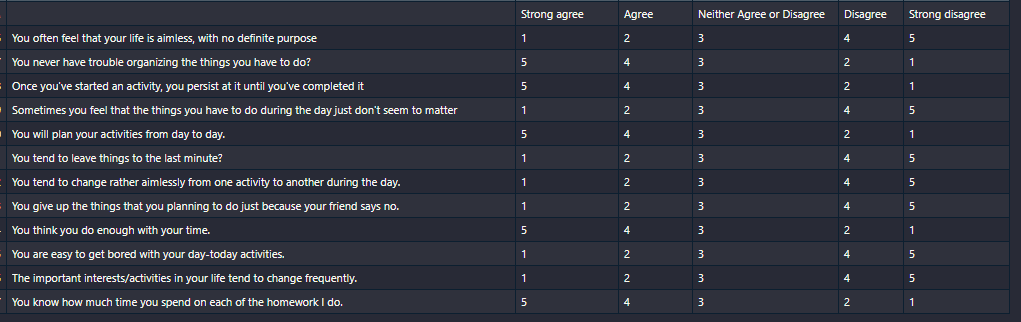
\includegraphics{q.png}
\caption{Les questions X6 à X17 et les types de réponse}
\end{figure}

\hypertarget{importation-des-donnuxe9es}{%
\subsection{Importation des données
:}\label{importation-des-donnuxe9es}}

Ici nous allons importer les données à partir du fichier csv, et
découvrir le dataset :

\begin{Shaded}
\begin{Highlighting}[]
\CommentTok{\# Importer les données}
\NormalTok{data }\OtherTok{\textless{}{-}} \FunctionTok{read.csv}\NormalTok{(}\StringTok{"International students Time management data.csv"}\NormalTok{)}

\CommentTok{\# Nombre de variables}
\FunctionTok{print}\NormalTok{(}\FunctionTok{ncol}\NormalTok{(data))}
\end{Highlighting}
\end{Shaded}

\begin{verbatim}
## [1] 21
\end{verbatim}

\begin{Shaded}
\begin{Highlighting}[]
\CommentTok{\# Nombre d\textquotesingle{}individus}
\FunctionTok{print}\NormalTok{(}\FunctionTok{nrow}\NormalTok{(data))}
\end{Highlighting}
\end{Shaded}

\begin{verbatim}
## [1] 125
\end{verbatim}

\begin{Shaded}
\begin{Highlighting}[]
\CommentTok{\# Le noms des variables}
\ControlFlowTok{for}\NormalTok{(i }\ControlFlowTok{in} \DecValTok{1}\SpecialCharTok{:}\FunctionTok{ncol}\NormalTok{(data))\{}
  \FunctionTok{print}\NormalTok{(}\FunctionTok{colnames}\NormalTok{(data)[i])}
\NormalTok{\}}
\end{Highlighting}
\end{Shaded}

\begin{verbatim}
## [1] "Number"
## [1] "Age"
## [1] "Gender"
## [1] "Nationality"
## [1] "Program"
## [1] "Course"
## [1] "English"
## [1] "Academic"
## [1] "Attendance"
## [1] "X6"
## [1] "X7"
## [1] "X8"
## [1] "X9"
## [1] "X10"
## [1] "X11"
## [1] "X12"
## [1] "X13"
## [1] "X14"
## [1] "X15"
## [1] "X16"
## [1] "X17"
\end{verbatim}

Donc on a 21 variables et 125 individus dans le dataset

\begin{figure}
\centering
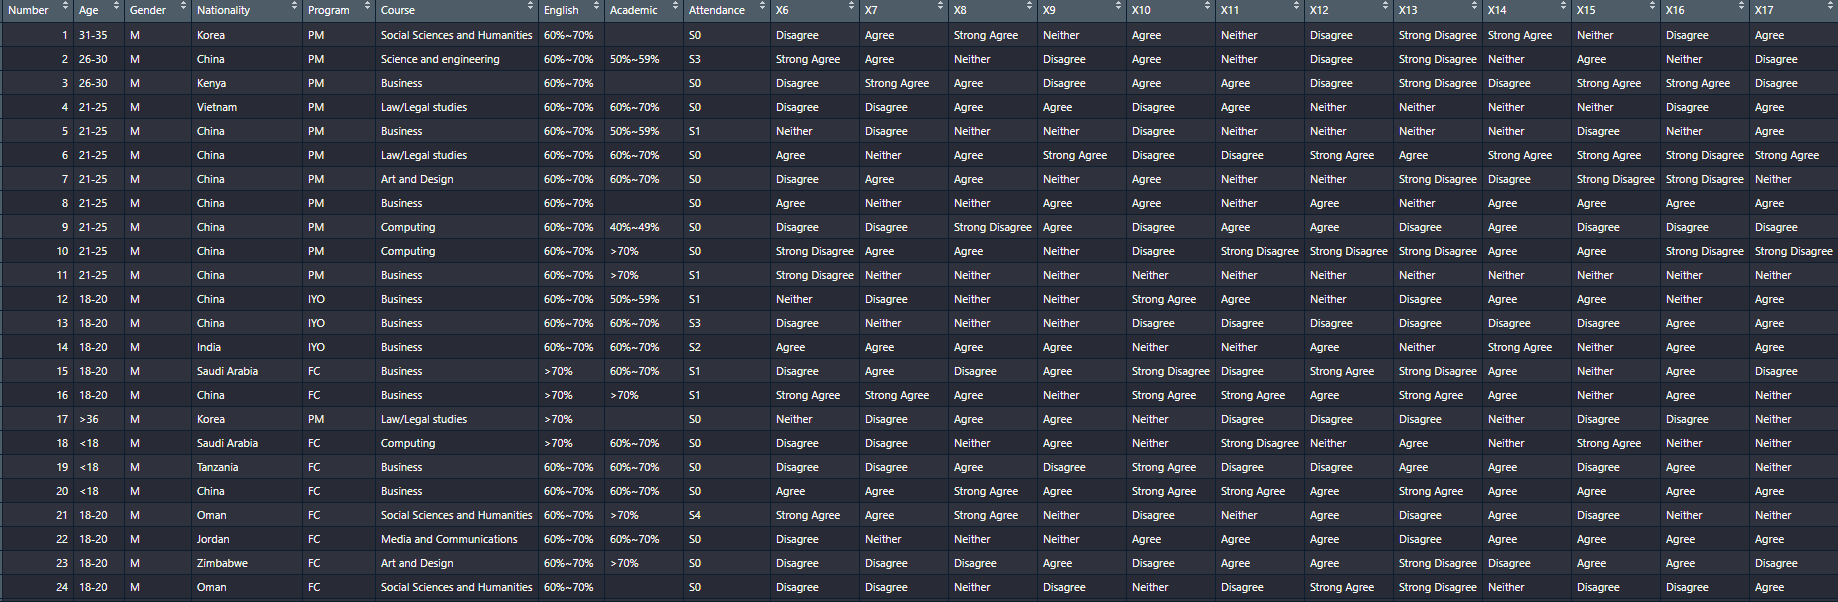
\includegraphics{d.png}
\caption{Overview du dataset}
\end{figure}

\hypertarget{pruxe9traitement-des-donnuxe9es}{%
\section{Prétraitement des données
:}\label{pruxe9traitement-des-donnuxe9es}}

On fait un summary pour voir les types des variables :

\begin{Shaded}
\begin{Highlighting}[]
\FunctionTok{summary}\NormalTok{(data)}
\end{Highlighting}
\end{Shaded}

\begin{verbatim}
##      Number        Age               Gender          Nationality       
##  Min.   :  1   Length:125         Length:125         Length:125        
##  1st Qu.: 32   Class :character   Class :character   Class :character  
##  Median : 63   Mode  :character   Mode  :character   Mode  :character  
##  Mean   : 63                                                           
##  3rd Qu.: 94                                                           
##  Max.   :125                                                           
##    Program             Course            English            Academic        
##  Length:125         Length:125         Length:125         Length:125        
##  Class :character   Class :character   Class :character   Class :character  
##  Mode  :character   Mode  :character   Mode  :character   Mode  :character  
##                                                                             
##                                                                             
##                                                                             
##   Attendance             X6                 X7                 X8           
##  Length:125         Length:125         Length:125         Length:125        
##  Class :character   Class :character   Class :character   Class :character  
##  Mode  :character   Mode  :character   Mode  :character   Mode  :character  
##                                                                             
##                                                                             
##                                                                             
##       X9                X10                X11                X12           
##  Length:125         Length:125         Length:125         Length:125        
##  Class :character   Class :character   Class :character   Class :character  
##  Mode  :character   Mode  :character   Mode  :character   Mode  :character  
##                                                                             
##                                                                             
##                                                                             
##      X13                X14                X15                X16           
##  Length:125         Length:125         Length:125         Length:125        
##  Class :character   Class :character   Class :character   Class :character  
##  Mode  :character   Mode  :character   Mode  :character   Mode  :character  
##                                                                             
##                                                                             
##                                                                             
##      X17           
##  Length:125        
##  Class :character  
##  Mode  :character  
##                    
##                    
## 
\end{verbatim}

La première variables Number est quantitative et elle représente
uniquement un numéro séquentiel pour désigner un individu, donc on doit
l'éliminer :

\begin{Shaded}
\begin{Highlighting}[]
\NormalTok{data}\SpecialCharTok{$}\NormalTok{Number }\OtherTok{\textless{}{-}} \ConstantTok{NULL}
\end{Highlighting}
\end{Shaded}

On a remarqué qu'il y a des valeurs manquantes dans nos données, on va
les détécter pour décider comment on va remédier à ce problème. D'abord
on vérifie s'il y a des valeurs de types NA dans chaque colonnes

\begin{Shaded}
\begin{Highlighting}[]
\ControlFlowTok{for}\NormalTok{ (i }\ControlFlowTok{in} \DecValTok{1}\SpecialCharTok{:} \FunctionTok{ncol}\NormalTok{(data))\{}
  \FunctionTok{print}\NormalTok{(}\FunctionTok{sum}\NormalTok{(}\FunctionTok{is.na}\NormalTok{(data[,i])))}
\NormalTok{\}}
\end{Highlighting}
\end{Shaded}

\begin{verbatim}
## [1] 0
## [1] 0
## [1] 0
## [1] 0
## [1] 0
## [1] 0
## [1] 0
## [1] 0
## [1] 0
## [1] 0
## [1] 0
## [1] 0
## [1] 0
## [1] 0
## [1] 0
## [1] 0
## [1] 0
## [1] 0
## [1] 0
## [1] 0
\end{verbatim}

On conclut qu'il n'y a pas de valeurs de type NA, donc on vérifie les
chaine de characters vide :

\begin{Shaded}
\begin{Highlighting}[]
\ControlFlowTok{for}\NormalTok{ (i }\ControlFlowTok{in} \DecValTok{1}\SpecialCharTok{:} \FunctionTok{ncol}\NormalTok{(data))\{}
  \FunctionTok{print}\NormalTok{(}\FunctionTok{c}\NormalTok{(}\FunctionTok{colnames}\NormalTok{(data)[i],}\FunctionTok{sum}\NormalTok{((data[,i] }\SpecialCharTok{==} \StringTok{""}\NormalTok{))}\SpecialCharTok{/}\FunctionTok{nrow}\NormalTok{(data)}\SpecialCharTok{*}\DecValTok{100}\NormalTok{))}
\NormalTok{\}}
\end{Highlighting}
\end{Shaded}

\begin{verbatim}
## [1] "Age" "0"  
## [1] "Gender" "0"     
## [1] "Nationality" "0"          
## [1] "Program" "0"      
## [1] "Course" "0"     
## [1] "English" "4.8"    
## [1] "Academic" "17.6"    
## [1] "Attendance" "4.8"       
## [1] "X6"  "1.6"
## [1] "X7" "0" 
## [1] "X8"  "3.2"
## [1] "X9"  "5.6"
## [1] "X10" "0.8"
## [1] "X11" "1.6"
## [1] "X12" "2.4"
## [1] "X13" "0"  
## [1] "X14" "0.8"
## [1] "X15" "0"  
## [1] "X16" "1.6"
## [1] "X17" "0.8"
\end{verbatim}

On remarque que la variable académique a un nombre important de valeurs
manquantes ( 17.6\%) par rapport aux autres variables. Nous allons opter
à remplacer les valeurs manquantes dans chaque variables avec le mode de
cette variable.Pour ce faire, on aura besoin d'une fonction qui retourne
le mode d'une colonne :

\begin{Shaded}
\begin{Highlighting}[]
\NormalTok{Mode }\OtherTok{\textless{}{-}} \ControlFlowTok{function}\NormalTok{(u)\{}
\NormalTok{  tmp }\OtherTok{\textless{}{-}} \FunctionTok{unique}\NormalTok{(u)}
\NormalTok{  tmp[}\FunctionTok{which.max}\NormalTok{(}\FunctionTok{tabulate}\NormalTok{(}\FunctionTok{match}\NormalTok{(u,tmp)))]}
\NormalTok{\}}

\CommentTok{\# Le mode de la colonne académique}
\FunctionTok{Mode}\NormalTok{(data}\SpecialCharTok{$}\NormalTok{Academic)}
\end{Highlighting}
\end{Shaded}

\begin{verbatim}
## [1] "60%~70%"
\end{verbatim}

Le remplissage des valeurs manquantes :

\begin{Shaded}
\begin{Highlighting}[]
\ControlFlowTok{for}\NormalTok{ (i }\ControlFlowTok{in} \DecValTok{1}\SpecialCharTok{:} \FunctionTok{ncol}\NormalTok{(data))\{}
\NormalTok{  data[data[,i] }\SpecialCharTok{==} \StringTok{""}\NormalTok{,i] }\OtherTok{\textless{}{-}} \FunctionTok{Mode}\NormalTok{(data[,i])}
\NormalTok{\}}
\end{Highlighting}
\end{Shaded}

On a nettoyé nos données avec succés, il n'y a plus de valeurs
manquantes :

\begin{Shaded}
\begin{Highlighting}[]
\ControlFlowTok{for}\NormalTok{ (i }\ControlFlowTok{in} \DecValTok{1}\SpecialCharTok{:} \FunctionTok{ncol}\NormalTok{(data))\{}
  \FunctionTok{print}\NormalTok{(}\FunctionTok{c}\NormalTok{(}\FunctionTok{colnames}\NormalTok{(data)[i],}\FunctionTok{sum}\NormalTok{((data[,i] }\SpecialCharTok{==} \StringTok{""}\NormalTok{))}\SpecialCharTok{/}\FunctionTok{nrow}\NormalTok{(data)}\SpecialCharTok{*}\DecValTok{100}\NormalTok{))}
\NormalTok{\}}
\end{Highlighting}
\end{Shaded}

\begin{verbatim}
## [1] "Age" "0"  
## [1] "Gender" "0"     
## [1] "Nationality" "0"          
## [1] "Program" "0"      
## [1] "Course" "0"     
## [1] "English" "0"      
## [1] "Academic" "0"       
## [1] "Attendance" "0"         
## [1] "X6" "0" 
## [1] "X7" "0" 
## [1] "X8" "0" 
## [1] "X9" "0" 
## [1] "X10" "0"  
## [1] "X11" "0"  
## [1] "X12" "0"  
## [1] "X13" "0"  
## [1] "X14" "0"  
## [1] "X15" "0"  
## [1] "X16" "0"  
## [1] "X17" "0"
\end{verbatim}

\hypertarget{etude-et-visualisation-des-statistiques-des-donnuxe9es}{%
\section{Etude et visualisation des statistiques des données
:}\label{etude-et-visualisation-des-statistiques-des-donnuxe9es}}

Dans cette section , nous allons commencer à explorer nos données en
étudiant les modalités de chaque variables. On aura besoin d'une
fonction qui va nous donner des graphes consisten pour chaque variables

\begin{Shaded}
\begin{Highlighting}[]
\NormalTok{Cat\_plot }\OtherTok{\textless{}{-}} \ControlFlowTok{function}\NormalTok{(y,title)\{}
\NormalTok{  n }\OtherTok{\textless{}{-}} \FunctionTok{table}\NormalTok{(y)}
  \FunctionTok{barplot}\NormalTok{(n,}\AttributeTok{las =} \DecValTok{2}\NormalTok{,}\AttributeTok{main=}\NormalTok{title,}\AttributeTok{ylab =} \StringTok{"Count"}\NormalTok{)}
  \FunctionTok{text}\NormalTok{(}\AttributeTok{x =}\NormalTok{n, }\AttributeTok{label =}\NormalTok{ n,}\AttributeTok{pos =} \DecValTok{1}\NormalTok{, }\AttributeTok{col =} \StringTok{"red"}\NormalTok{)}
  
\NormalTok{\}}
\end{Highlighting}
\end{Shaded}

\hypertarget{la-variable-age}{%
\subsection{La variable Age :}\label{la-variable-age}}

En regardant le graph ci-dessous, il est clair que la majorité des
personnes interrogées appartenaient au groupe d'âge 21-25 ans. Il y
avait 6 personnes de moins de 18 ans et 4 de plus de 36 ans.

\begin{Shaded}
\begin{Highlighting}[]
\FunctionTok{Cat\_plot}\NormalTok{(data}\SpecialCharTok{$}\NormalTok{Age,}\StringTok{"La répartiton de l\textquotesingle{}age dans cette étude"}\NormalTok{)}
\end{Highlighting}
\end{Shaded}

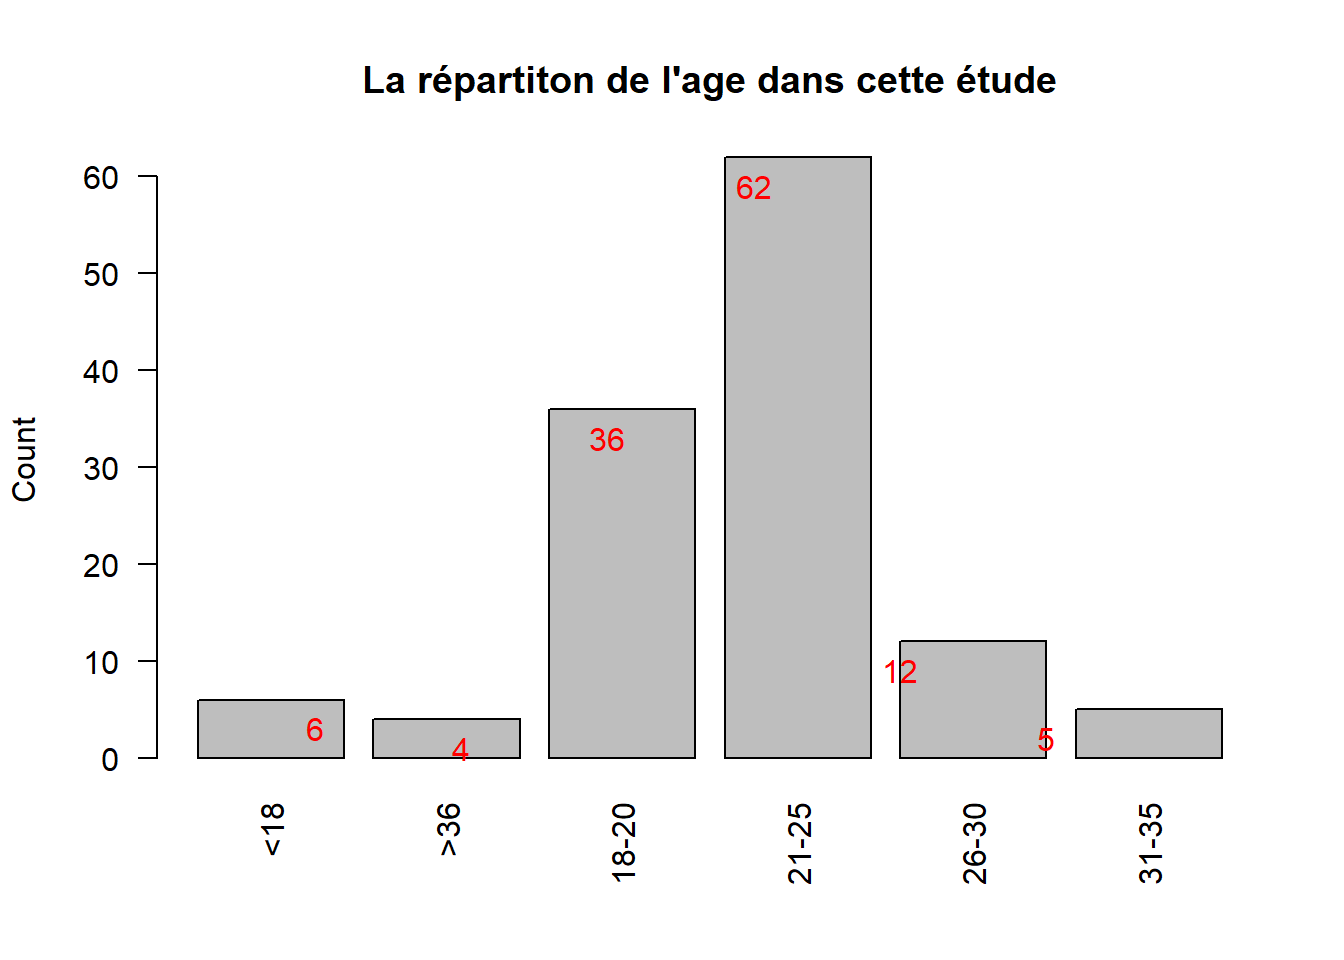
\includegraphics{AFCM_files/figure-latex/unnamed-chunk-10-1.pdf}

\hypertarget{la-variable-gender}{%
\subsection{La variable Gender :}\label{la-variable-gender}}

Il y avait une répartition presque égale entre les deux sexes dans
l'enquête, 63 femmes et 62 hommes.

\begin{Shaded}
\begin{Highlighting}[]
\FunctionTok{Cat\_plot}\NormalTok{(data}\SpecialCharTok{$}\NormalTok{Gender,}\StringTok{"La répartiton du sexe dans cette étude"}\NormalTok{)}
\end{Highlighting}
\end{Shaded}

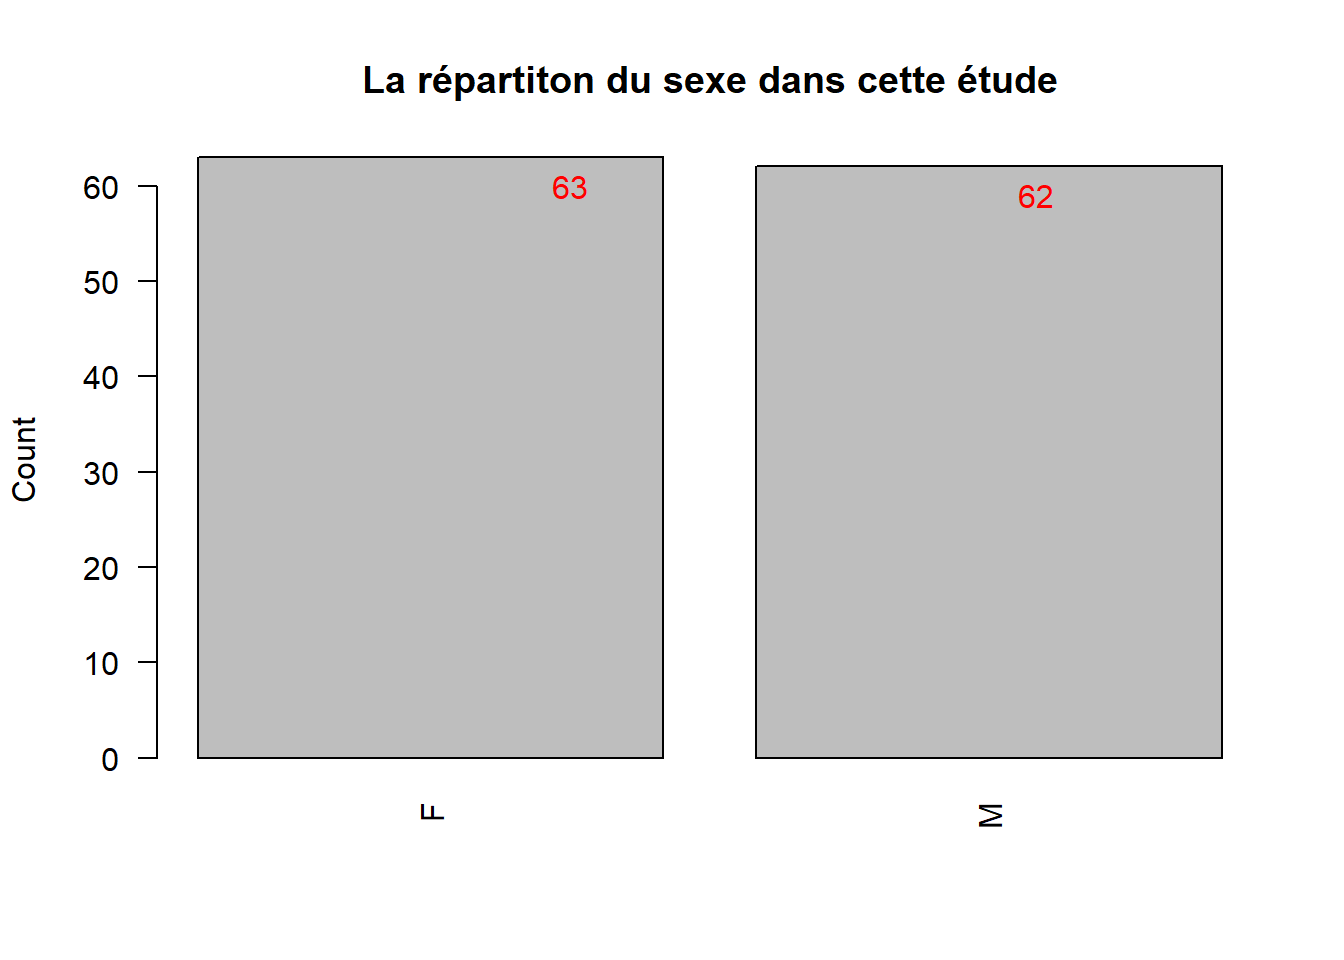
\includegraphics{AFCM_files/figure-latex/unnamed-chunk-11-1.pdf}

\hypertarget{la-variable-nationality}{%
\subsection{La variable Nationality}\label{la-variable-nationality}}

La majorité (77) des étudiants interrogés étaient chinois, suivis par
l'Arabie saoudite et la Corée à 6. La majorité des pays avaient 2 ou 1
étudiant interrogé.

\begin{Shaded}
\begin{Highlighting}[]
\FunctionTok{Cat\_plot}\NormalTok{(data}\SpecialCharTok{$}\NormalTok{Nationality,}\StringTok{"La répartiton de la nationalité dans cette étude"}\NormalTok{)}
\end{Highlighting}
\end{Shaded}

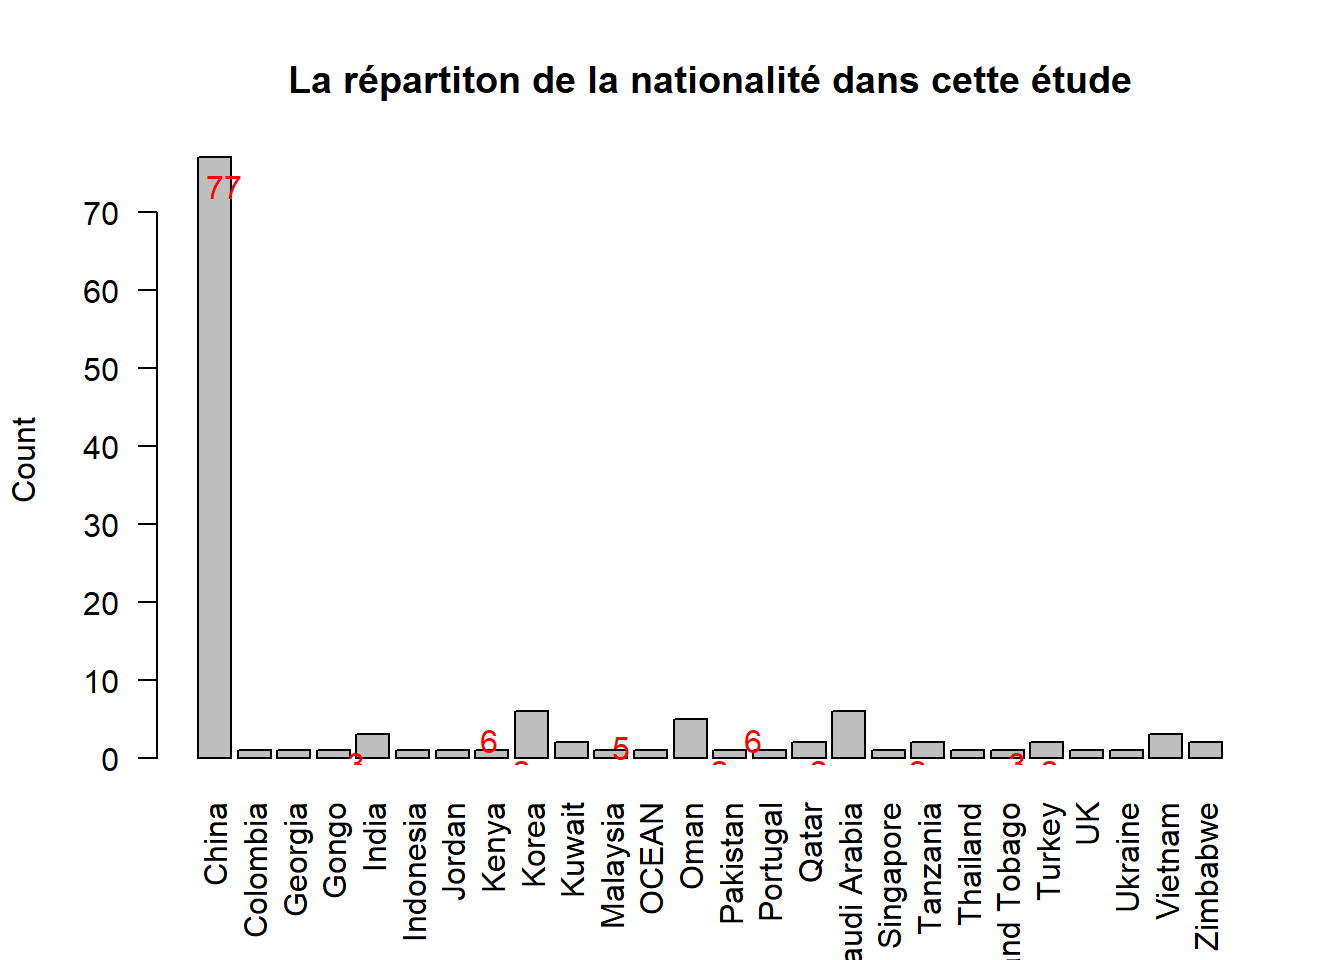
\includegraphics{AFCM_files/figure-latex/unnamed-chunk-12-1.pdf}

\hypertarget{la-variable-program}{%
\subsection{La variable Program :}\label{la-variable-program}}

La majorité des répondants au sondage étaient dans le programme PM,
suivi du programme FC à 31 étudiants. Le programme de langue n'avait
qu'un seul étudiant interrogé.

\begin{Shaded}
\begin{Highlighting}[]
\FunctionTok{Cat\_plot}\NormalTok{(data}\SpecialCharTok{$}\NormalTok{Program,}\StringTok{"La répartiton du Program dans cette étude"}\NormalTok{)}
\end{Highlighting}
\end{Shaded}

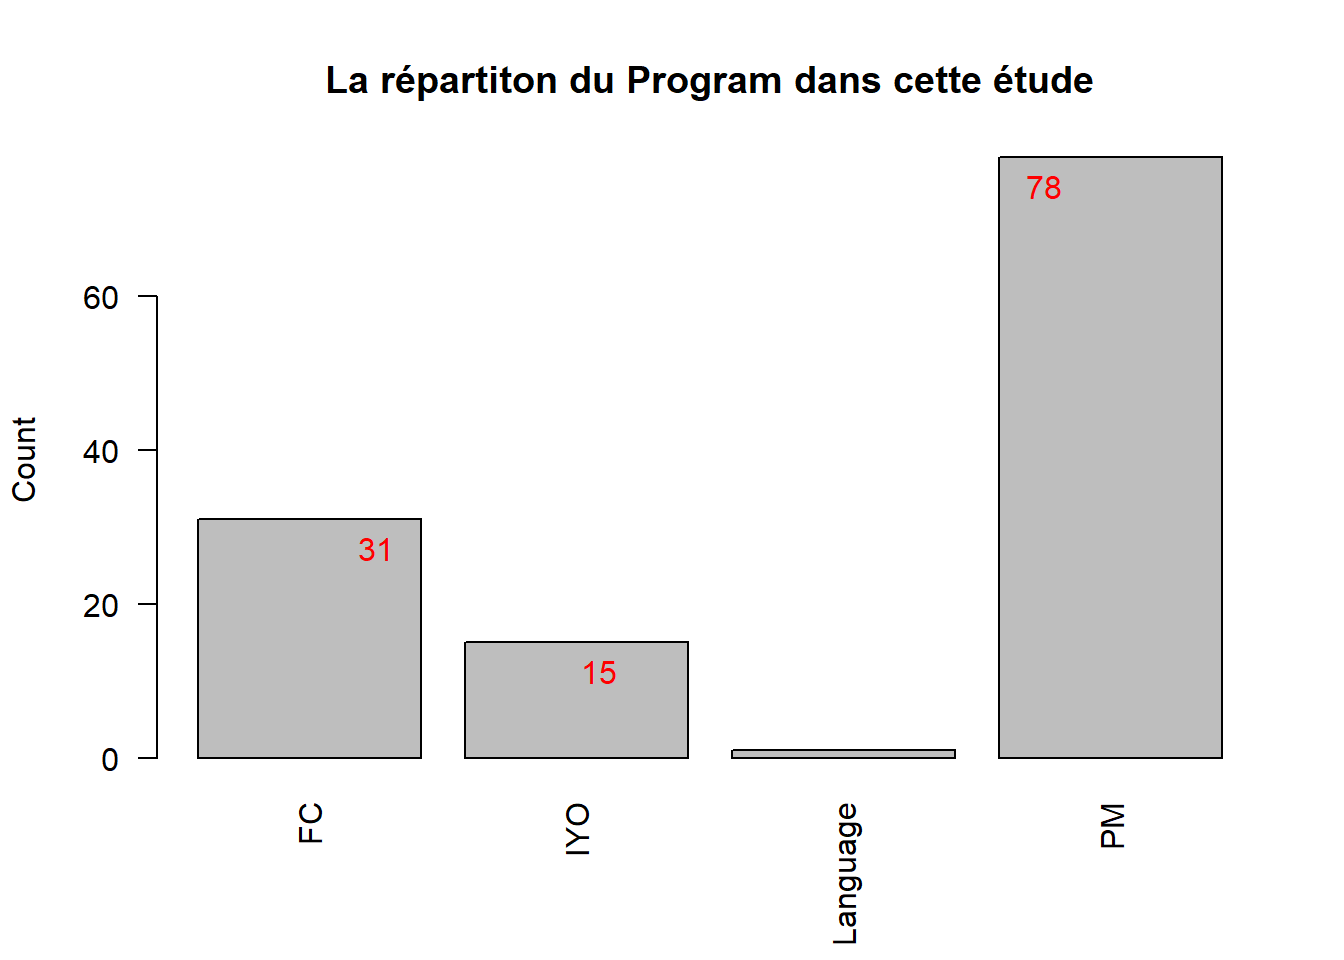
\includegraphics{AFCM_files/figure-latex/unnamed-chunk-13-1.pdf}

\hypertarget{la-variable-course}{%
\subsection{La variable Course :}\label{la-variable-course}}

La plupart des étudiants interrogés suivaient le cours du Business (80),
suivis de ceux du cours de Law/Legal Studies (14). Le cours sur Media
and Communications a le plus petit nombre d'étudiants interrogés à 3.

\begin{Shaded}
\begin{Highlighting}[]
\FunctionTok{Cat\_plot}\NormalTok{(data}\SpecialCharTok{$}\NormalTok{Course,}\StringTok{"La répartiton des Cours dans cette étude"}\NormalTok{)}
\end{Highlighting}
\end{Shaded}

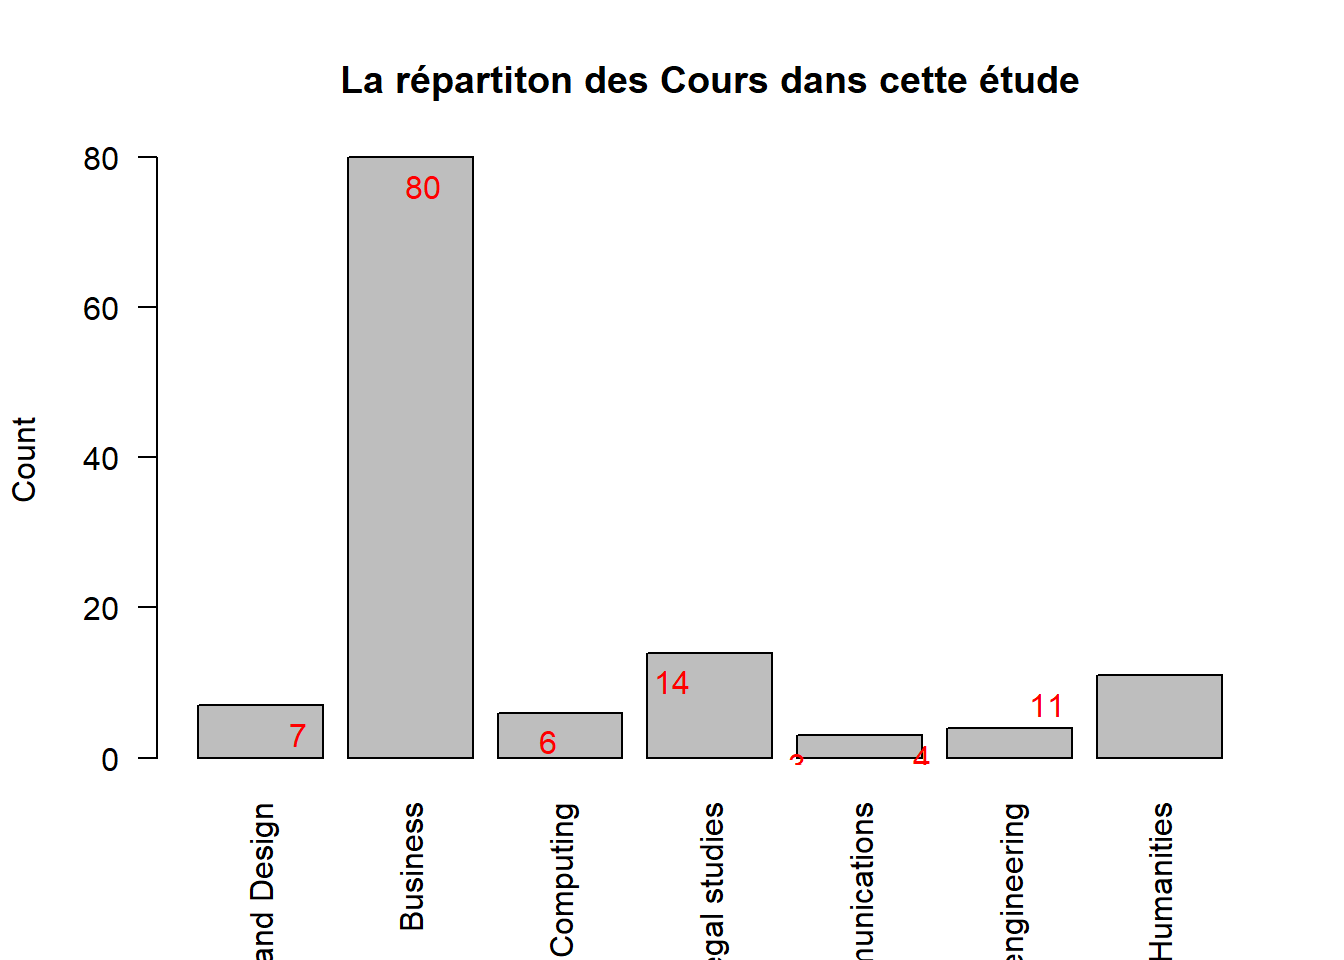
\includegraphics{AFCM_files/figure-latex/unnamed-chunk-14-1.pdf}

\hypertarget{la-variable-english}{%
\subsection{La variable English}\label{la-variable-english}}

Seuls 15 étudiants interrogés avaient des notes supérieures à 70\%, la
majorité des étudiants se situant entre 60 et 70\%. Il y avait une seule
personne qui était inférieure à 40 \%.

\begin{Shaded}
\begin{Highlighting}[]
\FunctionTok{Cat\_plot}\NormalTok{(data}\SpecialCharTok{$}\NormalTok{English,}\StringTok{"La répartiton du English  dans cette étude"}\NormalTok{)}
\end{Highlighting}
\end{Shaded}

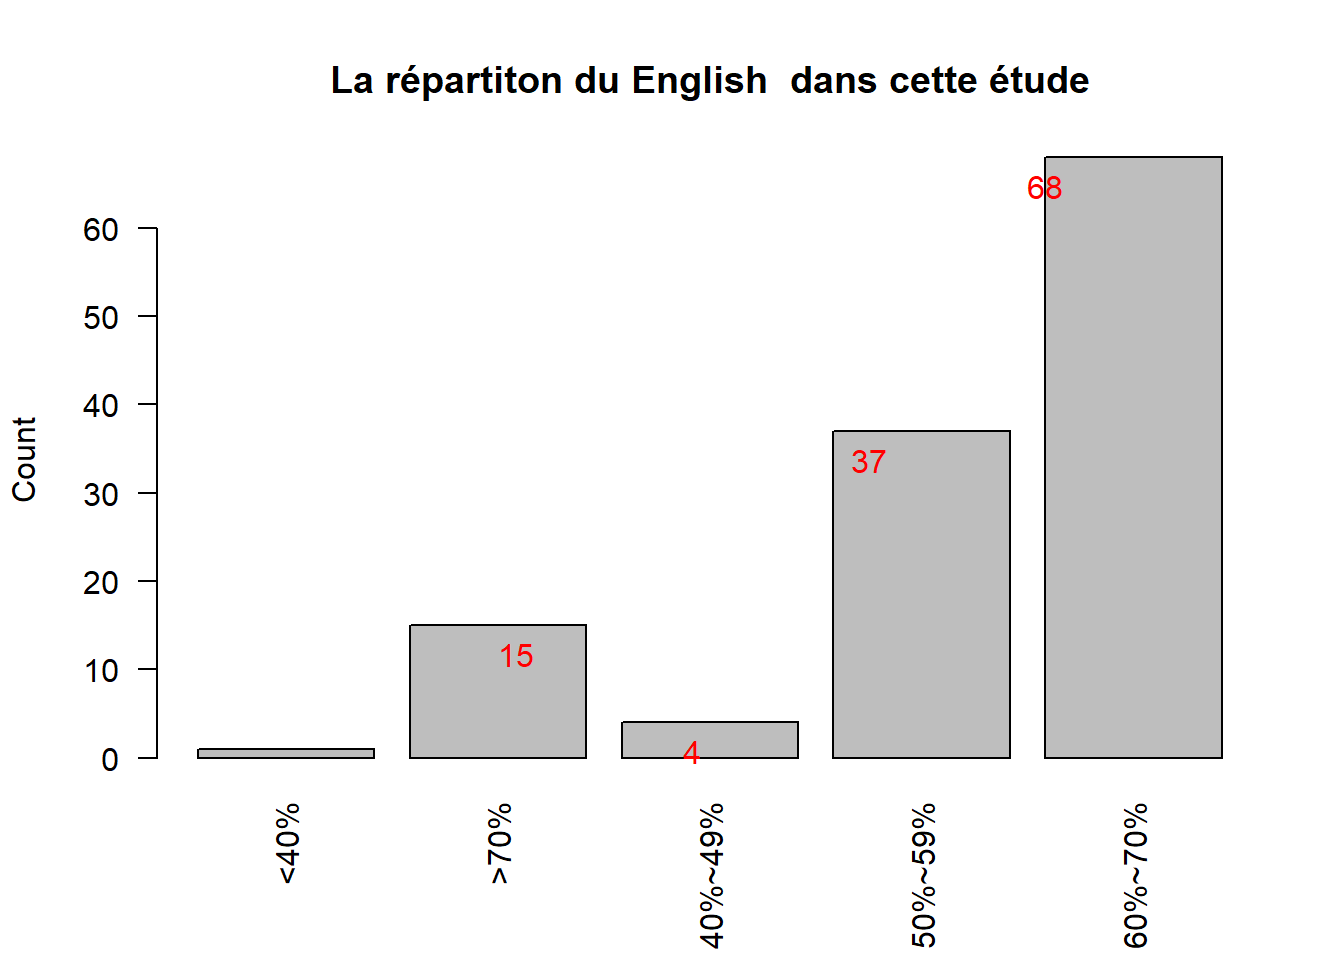
\includegraphics{AFCM_files/figure-latex/unnamed-chunk-15-1.pdf}

\hypertarget{la-variable-academic}{%
\subsection{La variable Academic :}\label{la-variable-academic}}

Les notes des cours académiques suivent un modèle similaire à ce que
nous avons vu avec les notes des cours d'anglais, la majorité des
étudiants interrogés se situent entre 60 et 70\%, 13 se situant entre
70\% et plus et2 avaient des notes inférieures à 40\%.

\begin{Shaded}
\begin{Highlighting}[]
\FunctionTok{Cat\_plot}\NormalTok{(data}\SpecialCharTok{$}\NormalTok{Academic,}\StringTok{"La répartiton du Academic dans cette étude"}\NormalTok{)}
\end{Highlighting}
\end{Shaded}

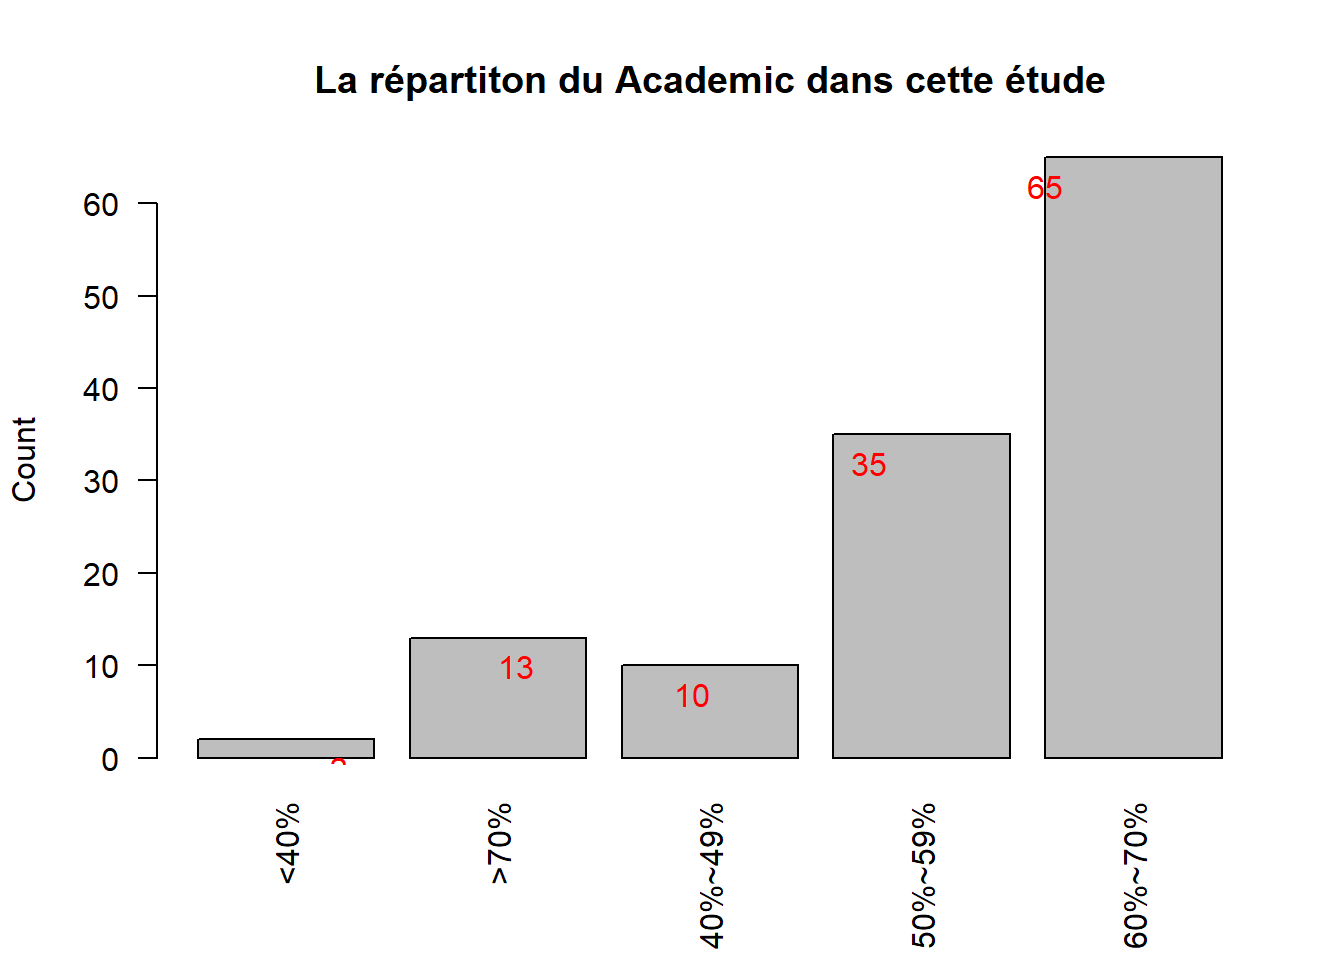
\includegraphics{AFCM_files/figure-latex/unnamed-chunk-16-1.pdf}

\hypertarget{la-variable-attendance}{%
\subsection{La variable Attendance :}\label{la-variable-attendance}}

La majorité des étudiants interrogés appartenaient au groupe S0 (63),
cela signifie que la plupart des étudiants avaient le plus de présence.

\begin{Shaded}
\begin{Highlighting}[]
\FunctionTok{Cat\_plot}\NormalTok{(data}\SpecialCharTok{$}\NormalTok{Attendance,}\StringTok{"La répartiton de l\textquotesingle{}Attendance dans cette étude"}\NormalTok{)}
\end{Highlighting}
\end{Shaded}

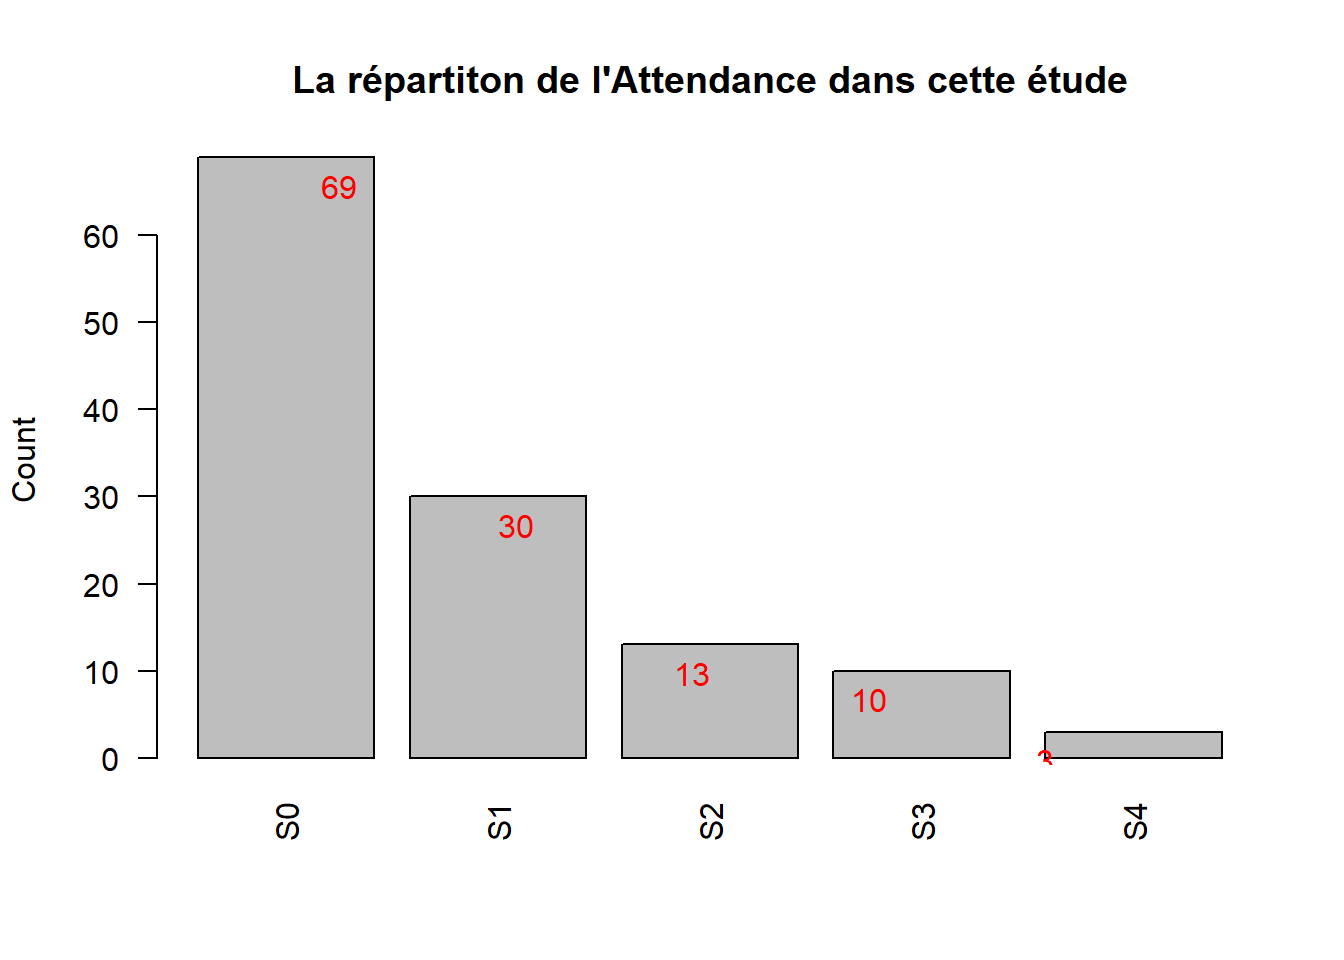
\includegraphics{AFCM_files/figure-latex/unnamed-chunk-17-1.pdf}

\hypertarget{la-variable-question-6}{%
\subsection{La variable question 6 :}\label{la-variable-question-6}}

50 étudiants interrogés sont en désaccord avec l'affirmation selon
laquelle leur vie est sans but, sans but précis, c'est la majorité. 23
étudiants interrogés étaient d'accord avec la déclaration, tandis que 27
étudiants n'avaient aucun sentiment dans les deux sens.

\begin{Shaded}
\begin{Highlighting}[]
\FunctionTok{Cat\_plot}\NormalTok{(data}\SpecialCharTok{$}\NormalTok{X6,}\StringTok{"La répartiton des réponse sur la question 6 dans cette étude"}\NormalTok{)}
\end{Highlighting}
\end{Shaded}

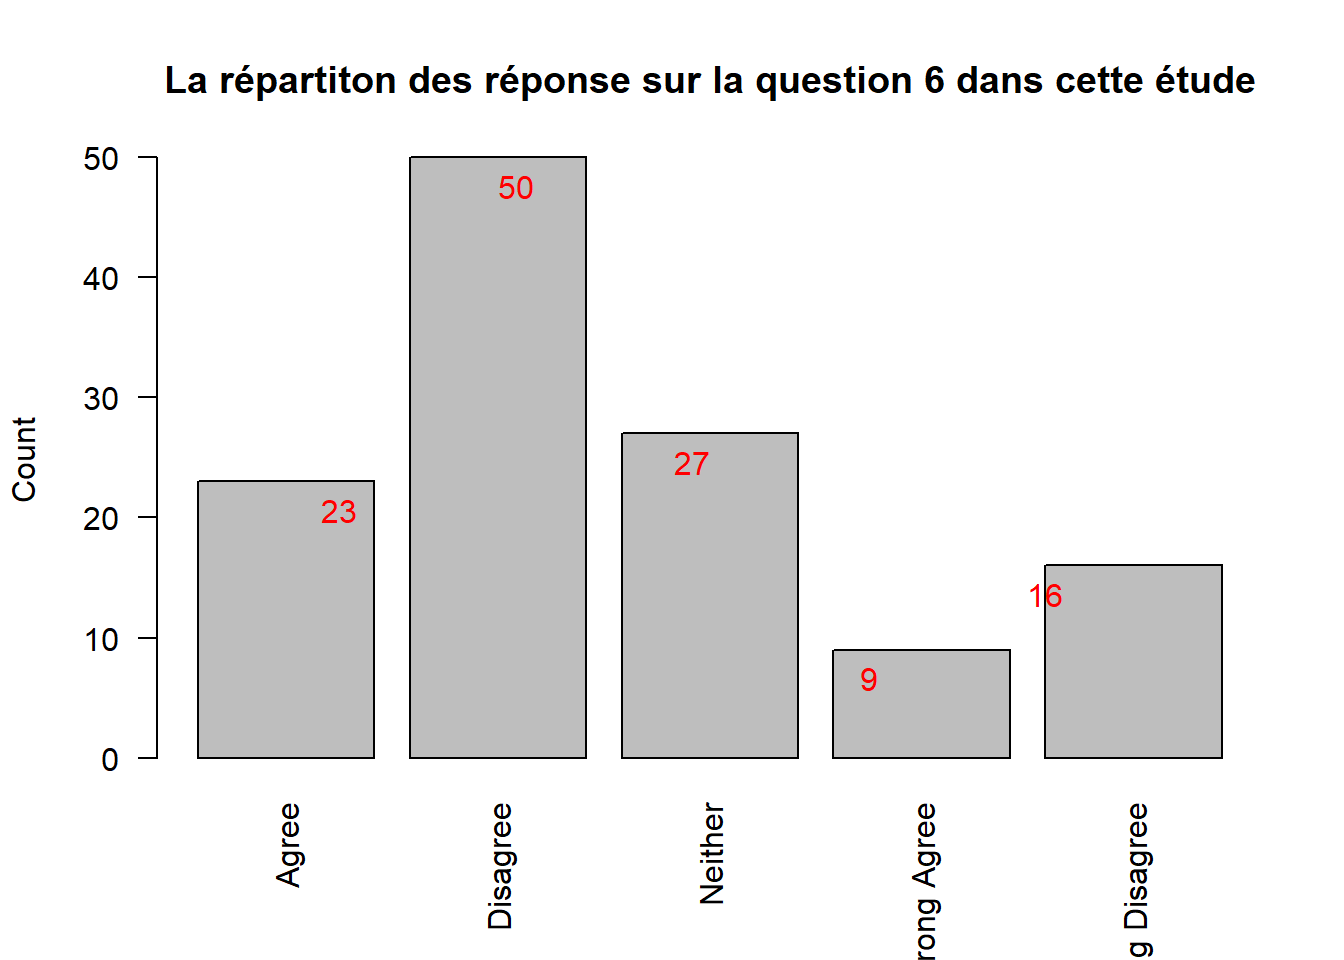
\includegraphics{AFCM_files/figure-latex/unnamed-chunk-18-1.pdf}

\hypertarget{la-variable-question-7}{%
\subsection{La variable question 7 :}\label{la-variable-question-7}}

40 étudiants interrogés ont déclaré qu'ils avaient du mal à organiser
les choses qu'ils ont à faire et 35 ont dit qu'ils n'avaient pas de mal.
Un total de 14 étudiants ont des sentiments forts dans les deux sens et
c'est une répartition égale dans les deux sens.

\begin{Shaded}
\begin{Highlighting}[]
\FunctionTok{Cat\_plot}\NormalTok{(data}\SpecialCharTok{$}\NormalTok{X7,}\StringTok{"La répartiton des réponse sur la question 7 dans cette étude"}\NormalTok{)}
\end{Highlighting}
\end{Shaded}

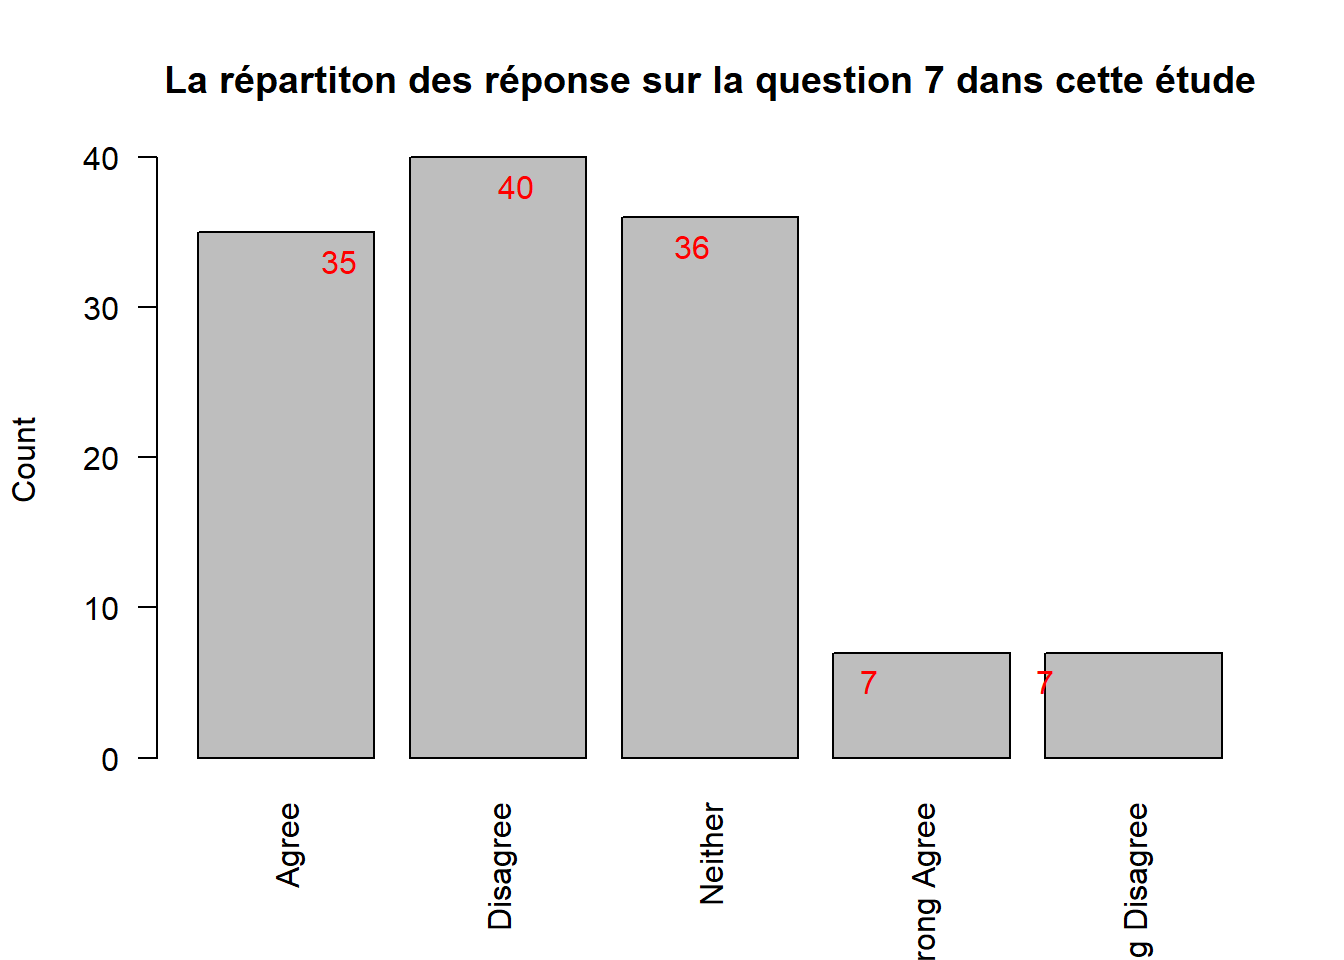
\includegraphics{AFCM_files/figure-latex/unnamed-chunk-19-1.pdf}

\hypertarget{la-variable-question-8}{%
\subsection{La variable question 8 :}\label{la-variable-question-8}}

61 étudiants interrogés ont déclaré qu'une fois qu'ils ont commencé
quelque chose, ils le finiront. Au total, 28 élèves ont déclaré qu'ils
étaient soit en désaccord soit fortement en désaccord quant à la fin des
activités qu'ils ont commencées.

\begin{Shaded}
\begin{Highlighting}[]
\FunctionTok{Cat\_plot}\NormalTok{(data}\SpecialCharTok{$}\NormalTok{X8,}\StringTok{"La répartiton des réponse sur la question 8 dans cette étude"}\NormalTok{)}
\end{Highlighting}
\end{Shaded}

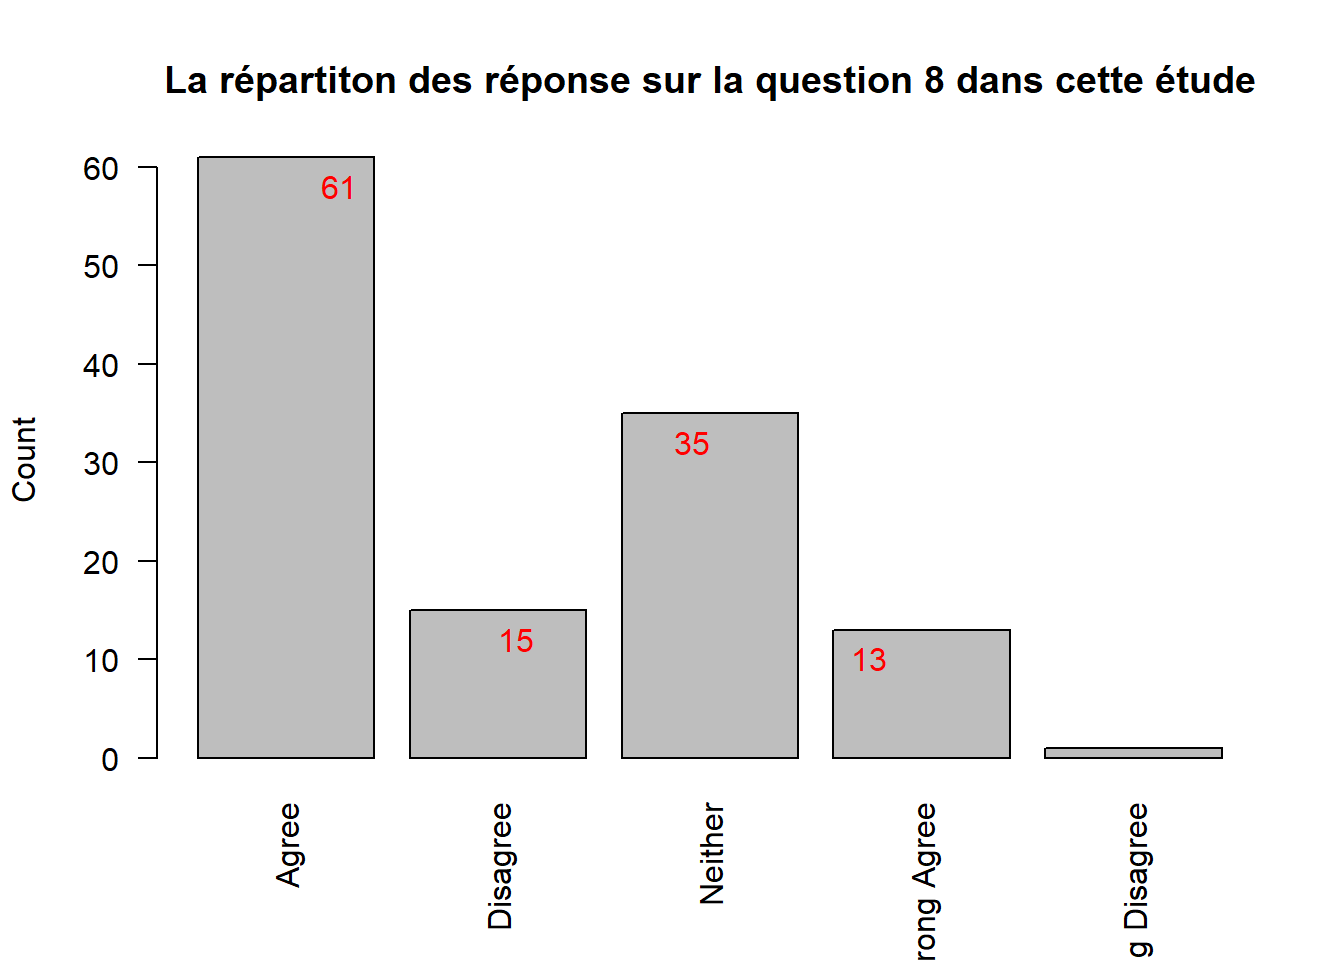
\includegraphics{AFCM_files/figure-latex/unnamed-chunk-20-1.pdf}

\hypertarget{la-variable-question-9}{%
\subsection{La variable question 9 :}\label{la-variable-question-9}}

44 étudiants interrogés étaient d'accord ou fortement d'accord qu'ils
ont parfois l'impression que les choses qu'ils doivent faire pendant la
journée n'ont tout simplement pas d'importance et 26 étudiants étaient
en désaccord ou fortement en désaccord. La majorité des étudiants (48)
n'ont répondu ni l'un ni l'autre.

\begin{Shaded}
\begin{Highlighting}[]
\FunctionTok{Cat\_plot}\NormalTok{(data}\SpecialCharTok{$}\NormalTok{X9,}\StringTok{"La répartiton des réponse sur la question 9 dans cette étude"}\NormalTok{)}
\end{Highlighting}
\end{Shaded}

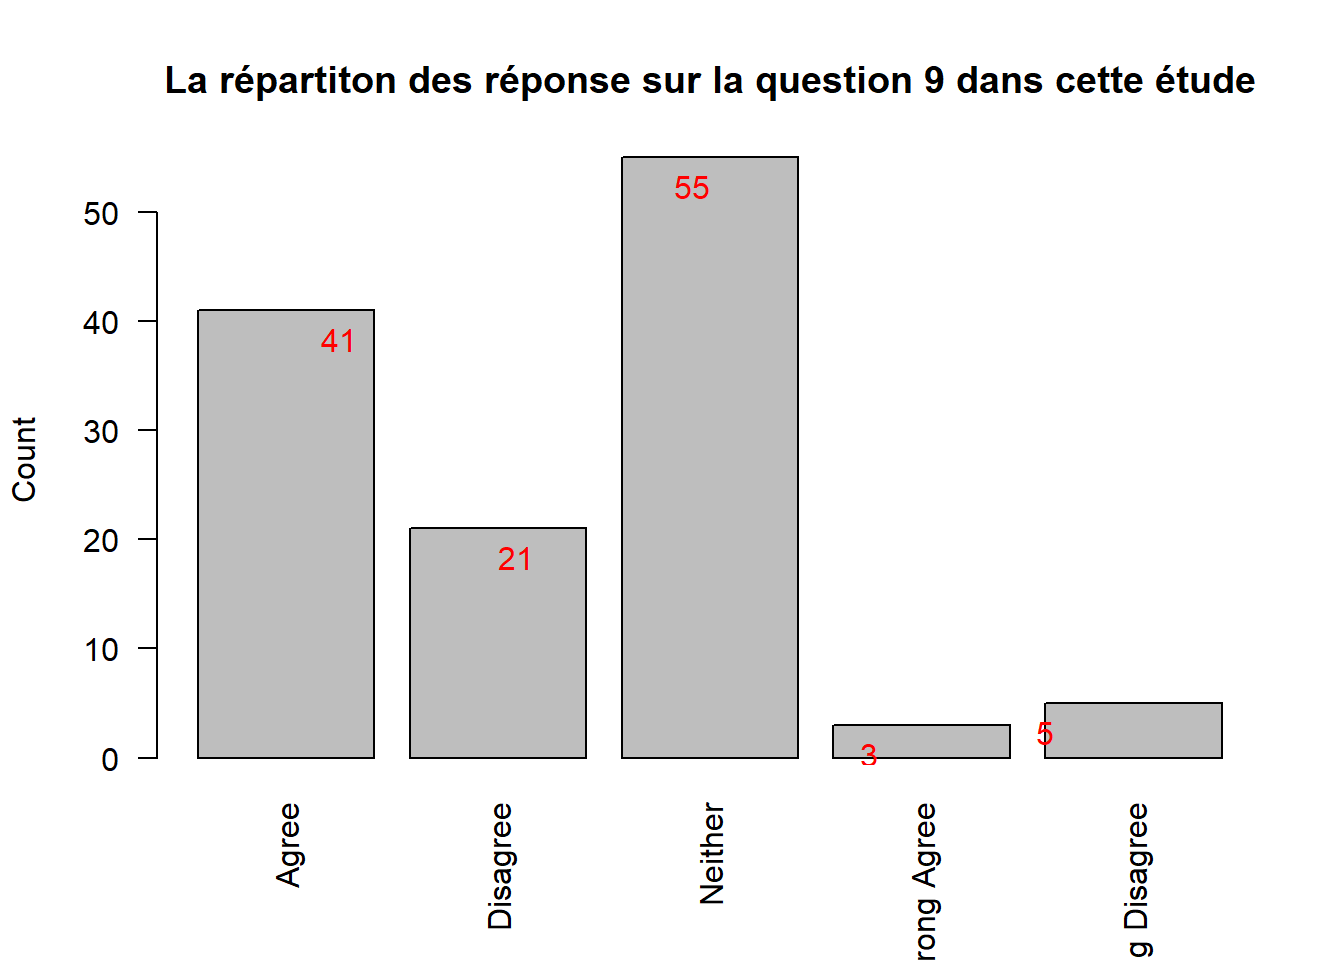
\includegraphics{AFCM_files/figure-latex/unnamed-chunk-21-1.pdf}

\hypertarget{la-variable-question-10}{%
\subsection{La variable question 10 :}\label{la-variable-question-10}}

Au total, 57 élèves ont déclaré être fortement d'accord ou d'accord avec
l'énoncé selon lequel ils planifient leurs activités. 34 élèves n'ont
répondu ni l'un ni l'autre.

\begin{Shaded}
\begin{Highlighting}[]
\FunctionTok{Cat\_plot}\NormalTok{(data}\SpecialCharTok{$}\NormalTok{X10,}\StringTok{"La répartiton des réponse sur la question 10 dans cette étude"}\NormalTok{)}
\end{Highlighting}
\end{Shaded}

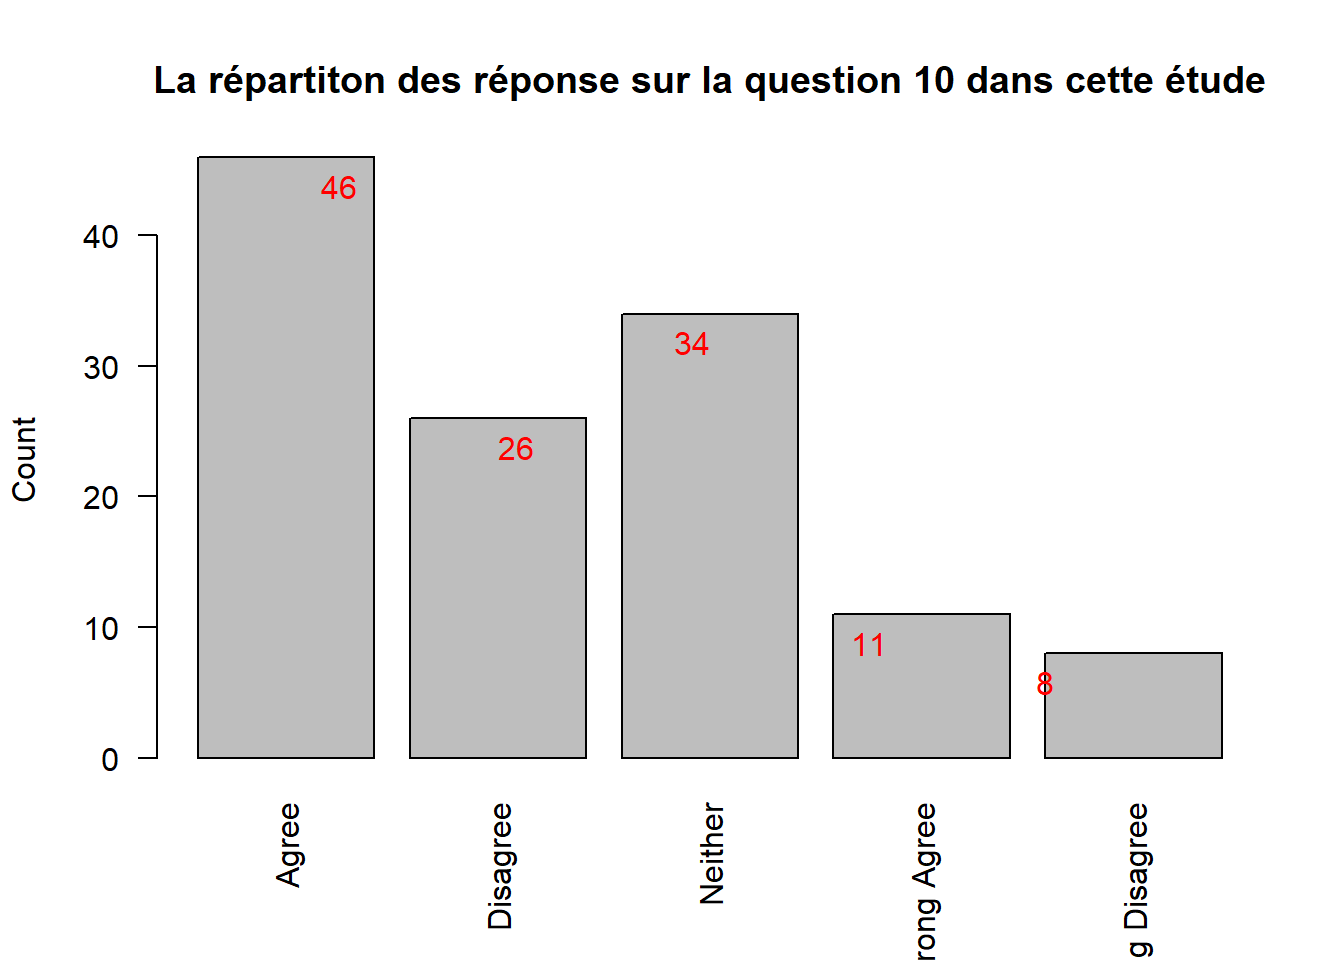
\includegraphics{AFCM_files/figure-latex/unnamed-chunk-22-1.pdf}

\hypertarget{la-variable-question-11}{%
\subsection{La variable question 11 :}\label{la-variable-question-11}}

La plupart des étudiants (38) ont déclaré qu'ils n'étaient pas d'accord
avec l'affirmation selon laquelle ils avaient laissé les choses à la
dernière minute. 31 ont dit qu'ils étaient d'accord pour laisser les
choses à la dernière minute.

\begin{Shaded}
\begin{Highlighting}[]
\FunctionTok{Cat\_plot}\NormalTok{(data}\SpecialCharTok{$}\NormalTok{X11,}\StringTok{"La répartiton des réponse sur la question 11 dans cette étude"}\NormalTok{)}
\end{Highlighting}
\end{Shaded}

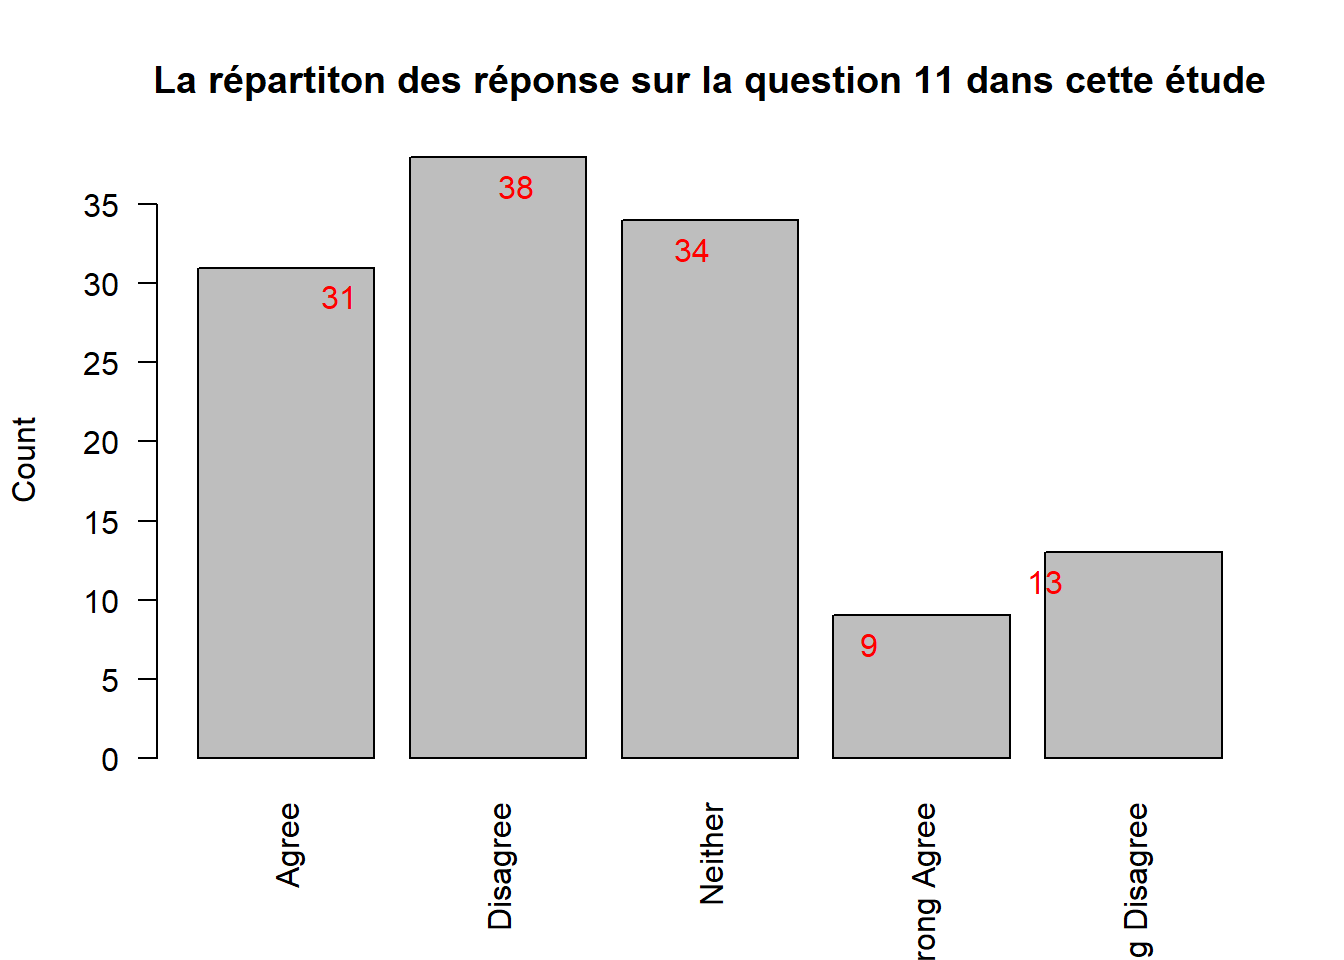
\includegraphics{AFCM_files/figure-latex/unnamed-chunk-23-1.pdf}

\hypertarget{la-variable-question-12}{%
\subsection{La variable question 12 :}\label{la-variable-question-12}}

52 étudiants ont déclaré qu'ils n'avaient pas tendance à passer sans but
précis d'une activité à l'autre au cours de la journée, c'est le nombre
le plus élevé parmi tous les choix possibles. Plus d'élèves étaient
d'accord/tout à fait d'accord qu'en désaccord/pas du tout d'accord avec
l'énoncé selon lequel ils ont tendance à passer sans but précis d'une
activité à l'autre au cours de la journée.

\begin{Shaded}
\begin{Highlighting}[]
\FunctionTok{Cat\_plot}\NormalTok{(data}\SpecialCharTok{$}\NormalTok{X12,}\StringTok{"La répartiton des réponse sur la question 12 dans cette étude"}\NormalTok{)}
\end{Highlighting}
\end{Shaded}

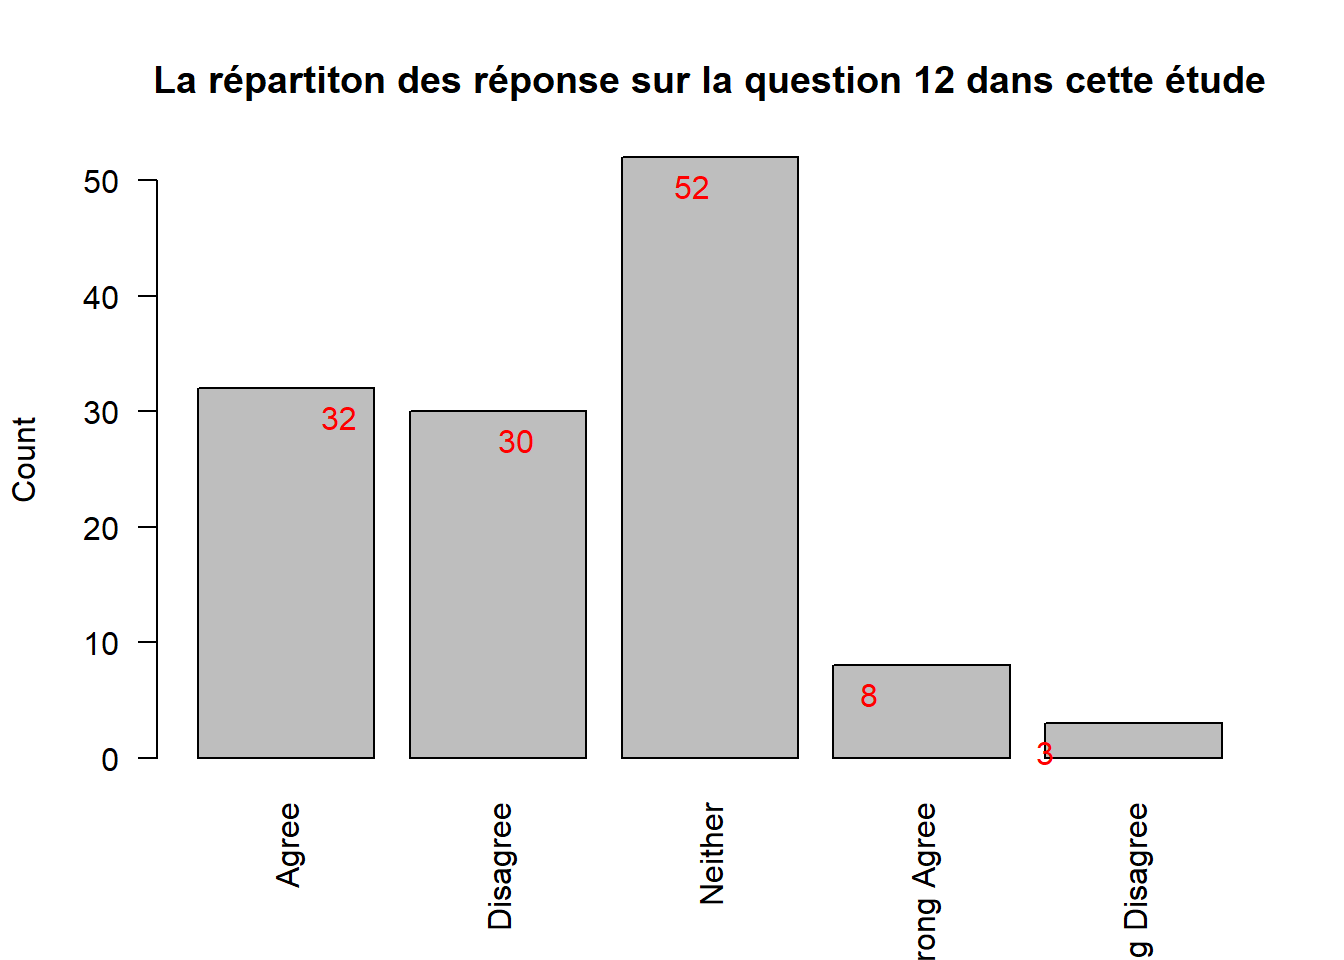
\includegraphics{AFCM_files/figure-latex/unnamed-chunk-24-1.pdf}

\hypertarget{la-variable-question-13}{%
\subsection{La variable question 13 :}\label{la-variable-question-13}}

Plus d'étudiants (42 + 39 = 81) ont dit qu'ils étaient en désaccord/pas
du tout d'accord que d'accord/tout à fait d'accord (13 + 5 = 18)
lorsqu'il s'agissait d'abandonner les choses qu'ils avaient prévu de
faire simplement parce que leur ami avait dit non.

\begin{Shaded}
\begin{Highlighting}[]
\FunctionTok{Cat\_plot}\NormalTok{(data}\SpecialCharTok{$}\NormalTok{X13,}\StringTok{"La répartiton des réponse sur la question 13 dans cette étude"}\NormalTok{)}
\end{Highlighting}
\end{Shaded}

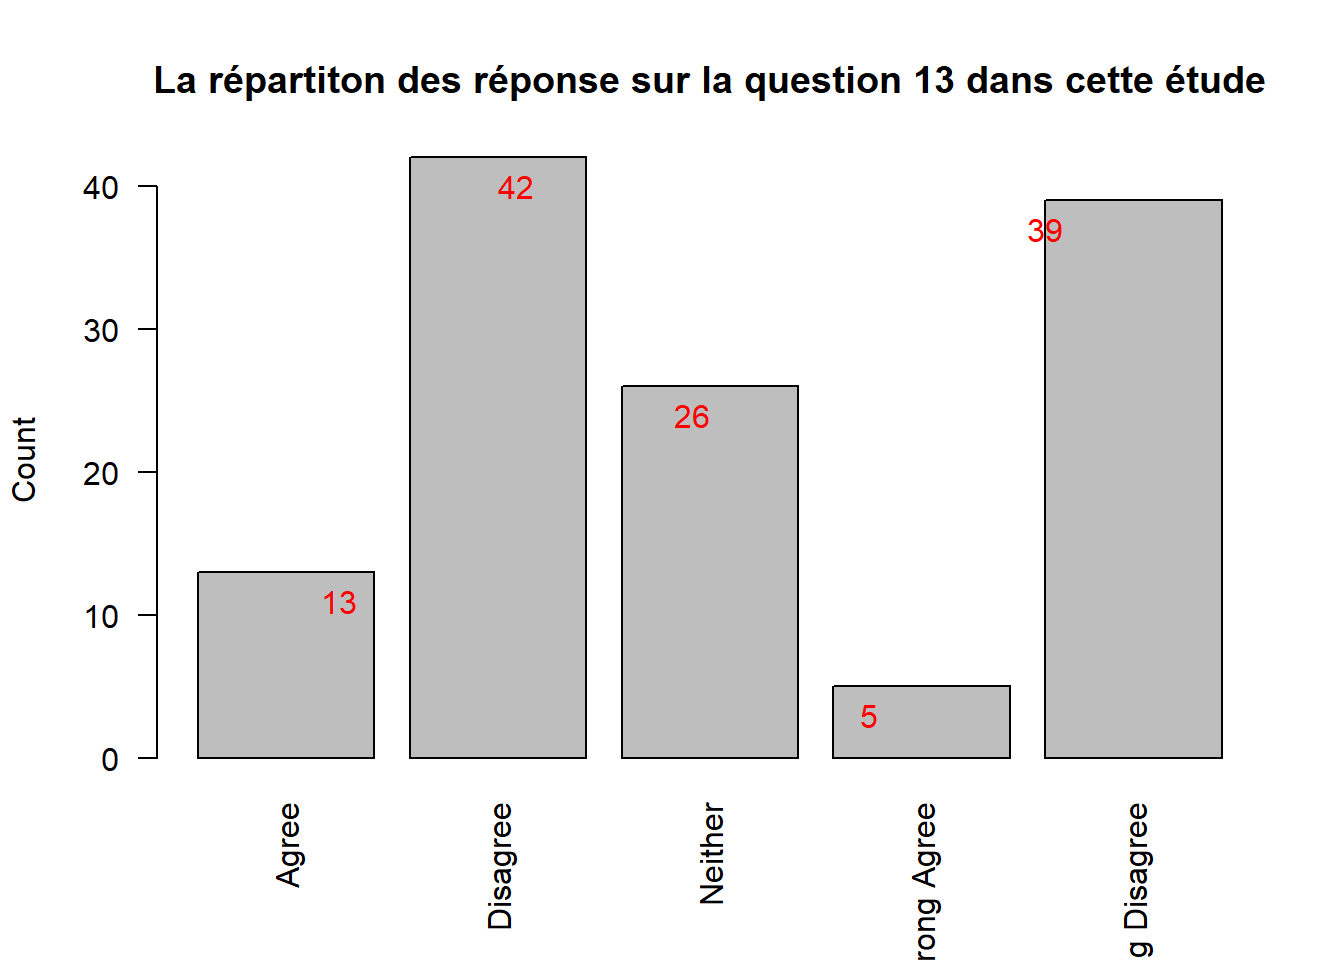
\includegraphics{AFCM_files/figure-latex/unnamed-chunk-25-1.pdf}

\hypertarget{la-variable-question-14}{%
\subsection{La variable question 14 :}\label{la-variable-question-14}}

47 étudiants étaient d'accord/tout à fait d'accord qu'ils avaient fait
assez de leur temps, et c'était la majorité des étudiants interrogés. 41
étudiants ont fait le chemin inverse avec leurs réponses et 37 n'ont dit
ni l'un ni l'autre.

\begin{Shaded}
\begin{Highlighting}[]
\FunctionTok{Cat\_plot}\NormalTok{(data}\SpecialCharTok{$}\NormalTok{X14,}\StringTok{"La répartiton des réponse sur la question 14 dans cette étude"}\NormalTok{)}
\end{Highlighting}
\end{Shaded}

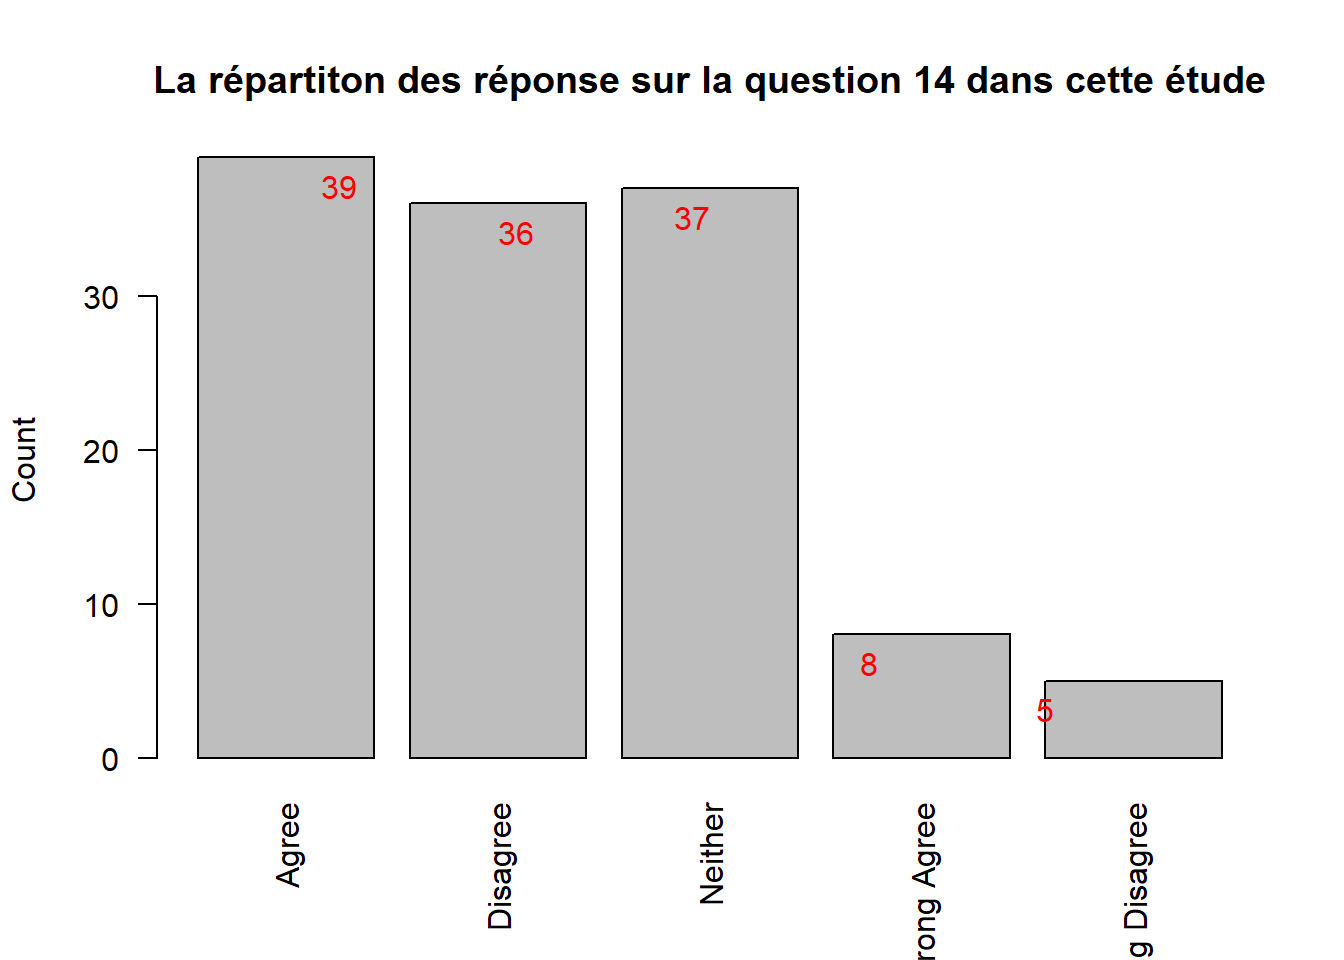
\includegraphics{AFCM_files/figure-latex/unnamed-chunk-26-1.pdf}

\hypertarget{la-variable-question-15}{%
\subsection{La variable question 15 :}\label{la-variable-question-15}}

La réponse la plus élevée à la question si les étudiants s'ennuient
facilement avec leurs activités quotidiennes d'aujourd'hui était la
réponse Neither avec 39 étudiants et est suivie par ceux qui étaient
d'accord (36) qu'ils s'ennuient facilement avec leurs activités
quotidiennes.

\begin{Shaded}
\begin{Highlighting}[]
\FunctionTok{Cat\_plot}\NormalTok{(data}\SpecialCharTok{$}\NormalTok{X15,}\StringTok{"La répartiton des réponse sur la question 15 dans cette étude"}\NormalTok{)}
\end{Highlighting}
\end{Shaded}

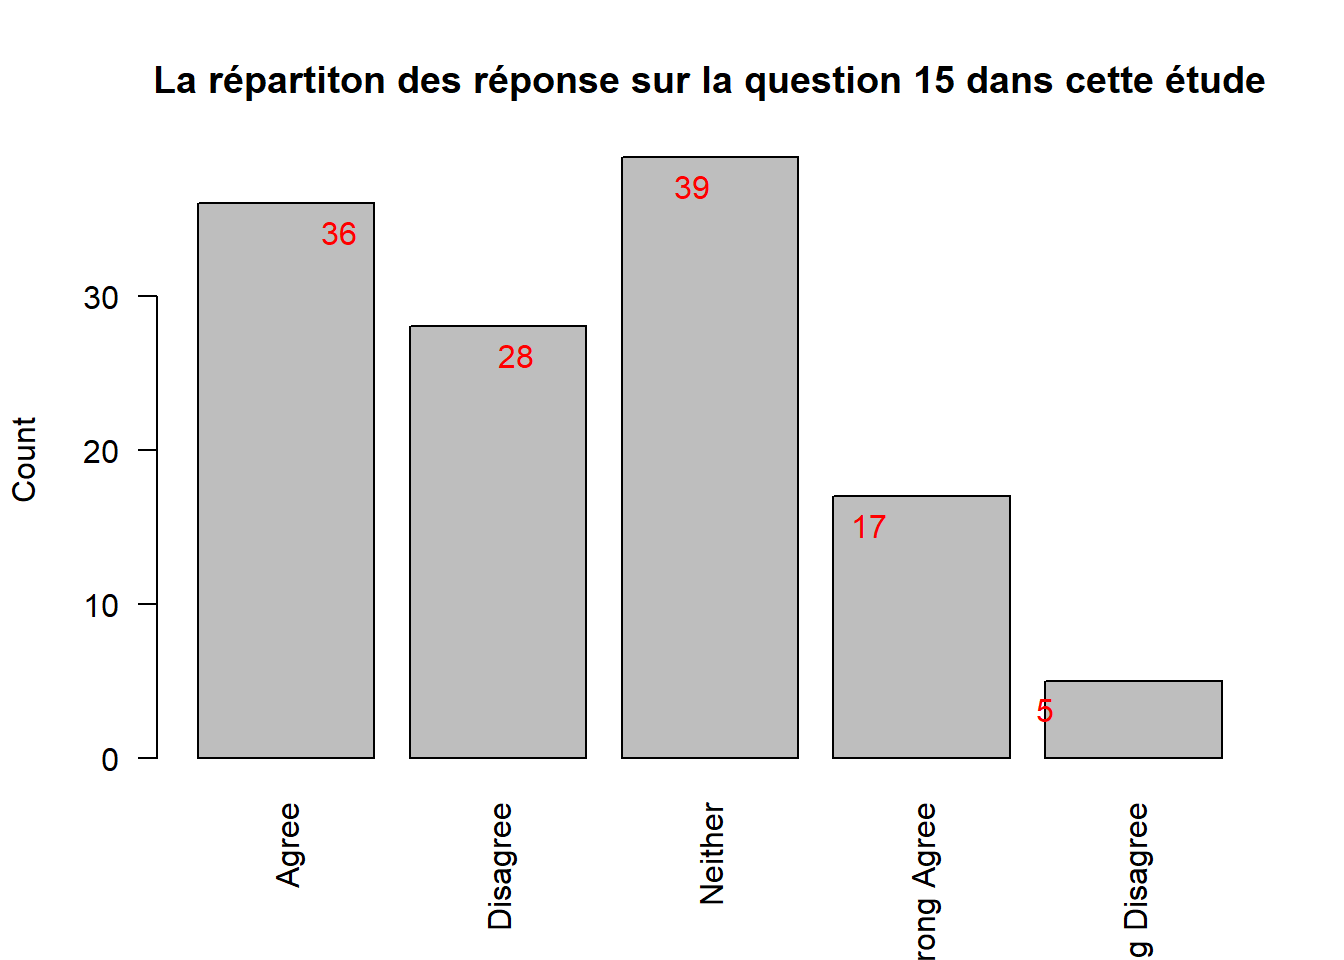
\includegraphics{AFCM_files/figure-latex/unnamed-chunk-27-1.pdf}

\hypertarget{la-variable-question-16}{%
\subsection{La variable question 16 :}\label{la-variable-question-16}}

47 étudiants ont déclaré que leurs intérêts/activités importants dans
leur vie avaient tendance à changer fréquemment. Cette réponse comptait
le plus grand nombre d'étudiants et était suivie par ceux qui n'étaient
pas d'accord (31).

\begin{Shaded}
\begin{Highlighting}[]
\FunctionTok{Cat\_plot}\NormalTok{(data}\SpecialCharTok{$}\NormalTok{X16,}\StringTok{"La répartiton des réponse sur la question 16 dans cette étude"}\NormalTok{)}
\end{Highlighting}
\end{Shaded}

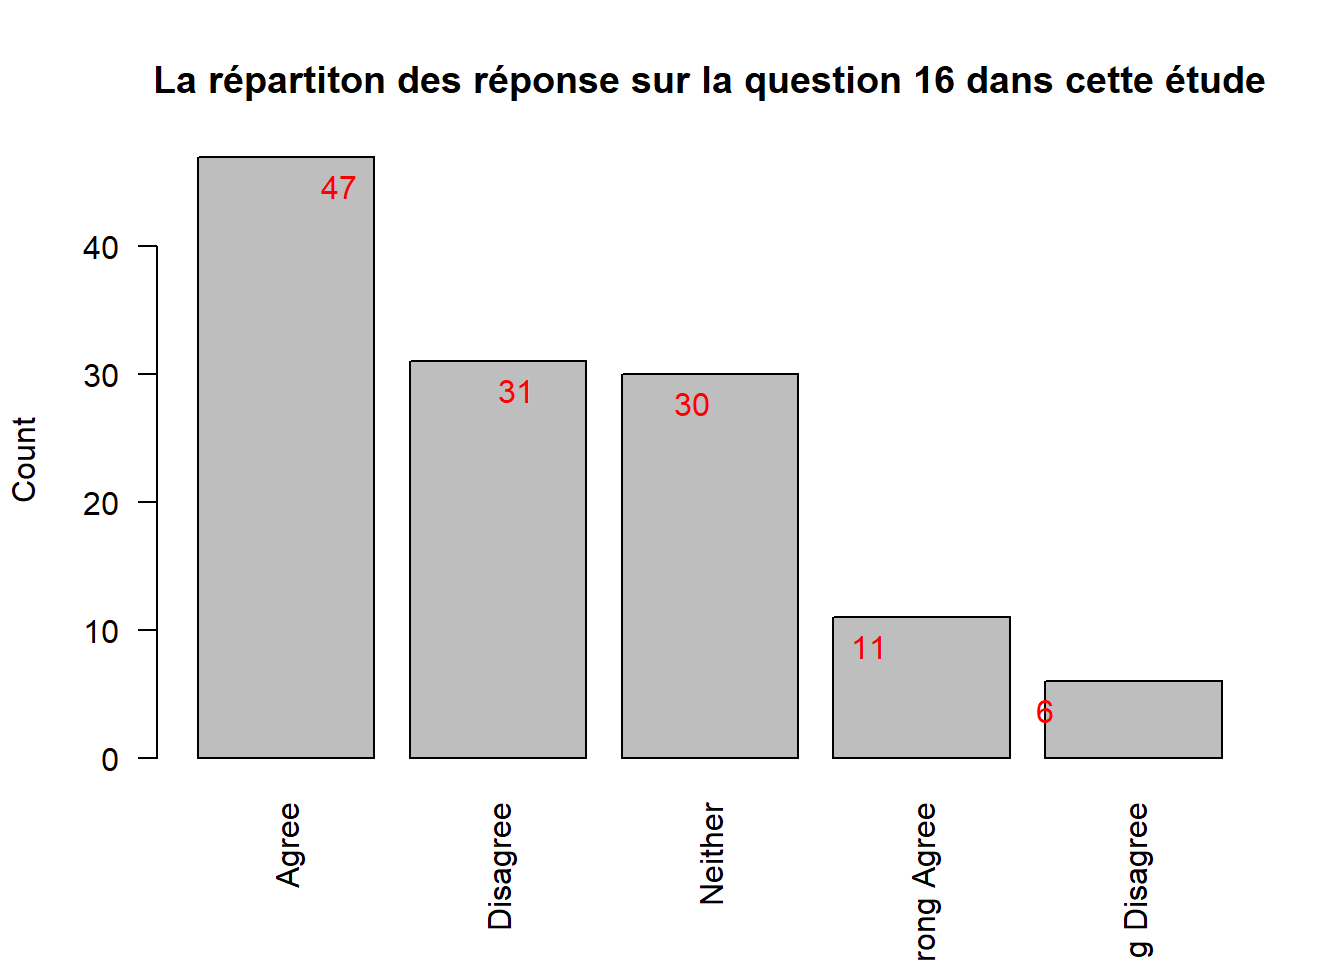
\includegraphics{AFCM_files/figure-latex/unnamed-chunk-28-1.pdf}

\hypertarget{la-variable-question-17}{%
\subsection{La variable question 17 :}\label{la-variable-question-17}}

Plus d'élèves étaient d'accord (45) que pas d'accord (29) avec l'énoncé
selon lequel ils savent combien de temps ils consacrent aux devoirs
qu'ils font.

\begin{Shaded}
\begin{Highlighting}[]
\FunctionTok{Cat\_plot}\NormalTok{(data}\SpecialCharTok{$}\NormalTok{X17,}\StringTok{"La répartiton des réponse sur la question 17 dans cette étude"}\NormalTok{)}
\end{Highlighting}
\end{Shaded}

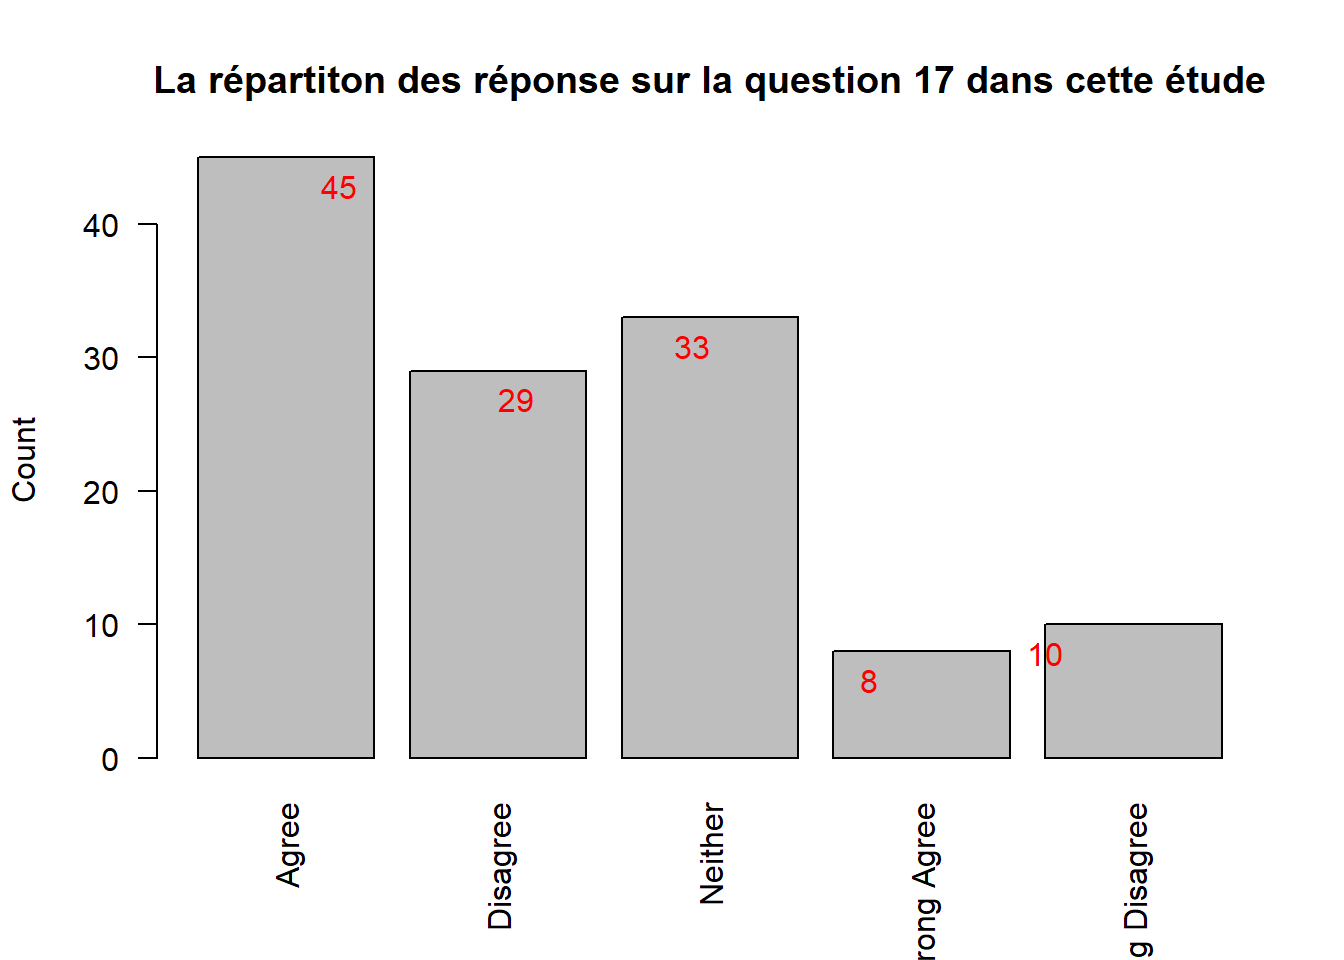
\includegraphics{AFCM_files/figure-latex/unnamed-chunk-29-1.pdf}

\hypertarget{pruxe9paration-uxe0-lafcm}{%
\section{Préparation à l'AFCm}\label{pruxe9paration-uxe0-lafcm}}

Pour faire l'AFCM ou l'AFC il faut charger le package FactoMineR :

\begin{Shaded}
\begin{Highlighting}[]
\FunctionTok{library}\NormalTok{(FactoMineR)}
\FunctionTok{library}\NormalTok{(factoextra)}
\end{Highlighting}
\end{Shaded}

\begin{verbatim}
## Loading required package: ggplot2
\end{verbatim}

\begin{verbatim}
## Welcome! Want to learn more? See two factoextra-related books at https://goo.gl/ve3WBa
\end{verbatim}

On a remarqué que la variable nationality possède un nombre de modalité
important par rapport aux autres variables, donc on va l'éliminer, Aussi
quelques variables ont le meme nom des modalités donc nous allons les
renommer . Et pour pouvoir transformer notre dataset à un tableau
disjonctif complet, il faut d'abord transformer les colonnes au type
factor :

\begin{Shaded}
\begin{Highlighting}[]
\NormalTok{data}\SpecialCharTok{$}\NormalTok{Nationality }\OtherTok{\textless{}{-}} \ConstantTok{NULL}

\NormalTok{data}\SpecialCharTok{$}\NormalTok{English }\OtherTok{\textless{}{-}} \FunctionTok{paste}\NormalTok{(}\StringTok{"English"}\NormalTok{,data}\SpecialCharTok{$}\NormalTok{English,}\AttributeTok{sep =}\StringTok{"\_"}\NormalTok{)}
\NormalTok{data}\SpecialCharTok{$}\NormalTok{Academic }\OtherTok{\textless{}{-}} \FunctionTok{paste}\NormalTok{(}\StringTok{"Academic"}\NormalTok{,data}\SpecialCharTok{$}\NormalTok{Academic,}\AttributeTok{sep =}\StringTok{"\_"}\NormalTok{)}
\NormalTok{data}\SpecialCharTok{$}\NormalTok{X6 }\OtherTok{\textless{}{-}} \FunctionTok{paste}\NormalTok{(}\StringTok{"X6"}\NormalTok{,data}\SpecialCharTok{$}\NormalTok{X6,}\AttributeTok{sep =} \StringTok{"\_"}\NormalTok{)}
\NormalTok{data}\SpecialCharTok{$}\NormalTok{X7 }\OtherTok{\textless{}{-}} \FunctionTok{paste}\NormalTok{(}\StringTok{"X7"}\NormalTok{,data}\SpecialCharTok{$}\NormalTok{X7,}\AttributeTok{sep =}\StringTok{"\_"}\NormalTok{)}
\NormalTok{data}\SpecialCharTok{$}\NormalTok{X8 }\OtherTok{\textless{}{-}} \FunctionTok{paste}\NormalTok{(}\StringTok{"X8"}\NormalTok{,data}\SpecialCharTok{$}\NormalTok{X8,}\AttributeTok{sep =}\StringTok{"\_"}\NormalTok{)}
\NormalTok{data}\SpecialCharTok{$}\NormalTok{X9 }\OtherTok{\textless{}{-}} \FunctionTok{paste}\NormalTok{(}\StringTok{"X9"}\NormalTok{,data}\SpecialCharTok{$}\NormalTok{X9,}\AttributeTok{sep =}\StringTok{"\_"}\NormalTok{)}
\NormalTok{data}\SpecialCharTok{$}\NormalTok{X10 }\OtherTok{\textless{}{-}} \FunctionTok{paste}\NormalTok{(}\StringTok{"X10"}\NormalTok{,data}\SpecialCharTok{$}\NormalTok{X10,}\AttributeTok{sep =}\StringTok{"\_"}\NormalTok{)}
\NormalTok{data}\SpecialCharTok{$}\NormalTok{X11 }\OtherTok{\textless{}{-}} \FunctionTok{paste}\NormalTok{(}\StringTok{"X11"}\NormalTok{,data}\SpecialCharTok{$}\NormalTok{X11,}\AttributeTok{sep =}\StringTok{"\_"}\NormalTok{)}
\NormalTok{data}\SpecialCharTok{$}\NormalTok{X12 }\OtherTok{\textless{}{-}} \FunctionTok{paste}\NormalTok{(}\StringTok{"X12"}\NormalTok{,data}\SpecialCharTok{$}\NormalTok{X12,}\AttributeTok{sep =}\StringTok{"\_"}\NormalTok{)}
\NormalTok{data}\SpecialCharTok{$}\NormalTok{X13 }\OtherTok{\textless{}{-}} \FunctionTok{paste}\NormalTok{(}\StringTok{"X13"}\NormalTok{,data}\SpecialCharTok{$}\NormalTok{X13,}\AttributeTok{sep =}\StringTok{"\_"}\NormalTok{)}
\NormalTok{data}\SpecialCharTok{$}\NormalTok{X14 }\OtherTok{\textless{}{-}} \FunctionTok{paste}\NormalTok{(}\StringTok{"X14"}\NormalTok{,data}\SpecialCharTok{$}\NormalTok{X14,}\AttributeTok{sep =}\StringTok{"\_"}\NormalTok{)}
\NormalTok{data}\SpecialCharTok{$}\NormalTok{X15 }\OtherTok{\textless{}{-}} \FunctionTok{paste}\NormalTok{(}\StringTok{"X15"}\NormalTok{,data}\SpecialCharTok{$}\NormalTok{X15,}\AttributeTok{sep =}\StringTok{"\_"}\NormalTok{)}
\NormalTok{data}\SpecialCharTok{$}\NormalTok{X16 }\OtherTok{\textless{}{-}} \FunctionTok{paste}\NormalTok{(}\StringTok{"X16"}\NormalTok{,data}\SpecialCharTok{$}\NormalTok{X16,}\AttributeTok{sep =}\StringTok{"\_"}\NormalTok{)}
\NormalTok{data}\SpecialCharTok{$}\NormalTok{X17 }\OtherTok{\textless{}{-}} \FunctionTok{paste}\NormalTok{(}\StringTok{"X17"}\NormalTok{,data}\SpecialCharTok{$}\NormalTok{X17,}\AttributeTok{sep =}\StringTok{"\_"}\NormalTok{)}

\NormalTok{J }\OtherTok{\textless{}{-}} \DecValTok{0}

\ControlFlowTok{for}\NormalTok{(i }\ControlFlowTok{in} \DecValTok{1}\SpecialCharTok{:} \FunctionTok{ncol}\NormalTok{(data))\{}
\NormalTok{  data[,i] }\OtherTok{\textless{}{-}} \FunctionTok{as.factor}\NormalTok{(data[,i])}
\NormalTok{  J }\OtherTok{\textless{}{-}}\NormalTok{ J }\SpecialCharTok{+} \FunctionTok{length}\NormalTok{(}\FunctionTok{levels}\NormalTok{(data[,i]))}
\NormalTok{\}}

\FunctionTok{print}\NormalTok{(}\FunctionTok{c}\NormalTok{(}\StringTok{"Nombre total de modaliés : "}\NormalTok{ ,J))}
\end{Highlighting}
\end{Shaded}

\begin{verbatim}
## [1] "Nombre total de modaliés : " "94"
\end{verbatim}

\begin{Shaded}
\begin{Highlighting}[]
\NormalTok{tdc }\OtherTok{\textless{}{-}} \FunctionTok{tab.disjonctif}\NormalTok{(data)}
\NormalTok{df }\OtherTok{\textless{}{-}} \FunctionTok{as.data.frame}\NormalTok{(tdc)}
\end{Highlighting}
\end{Shaded}

\begin{figure}
\centering
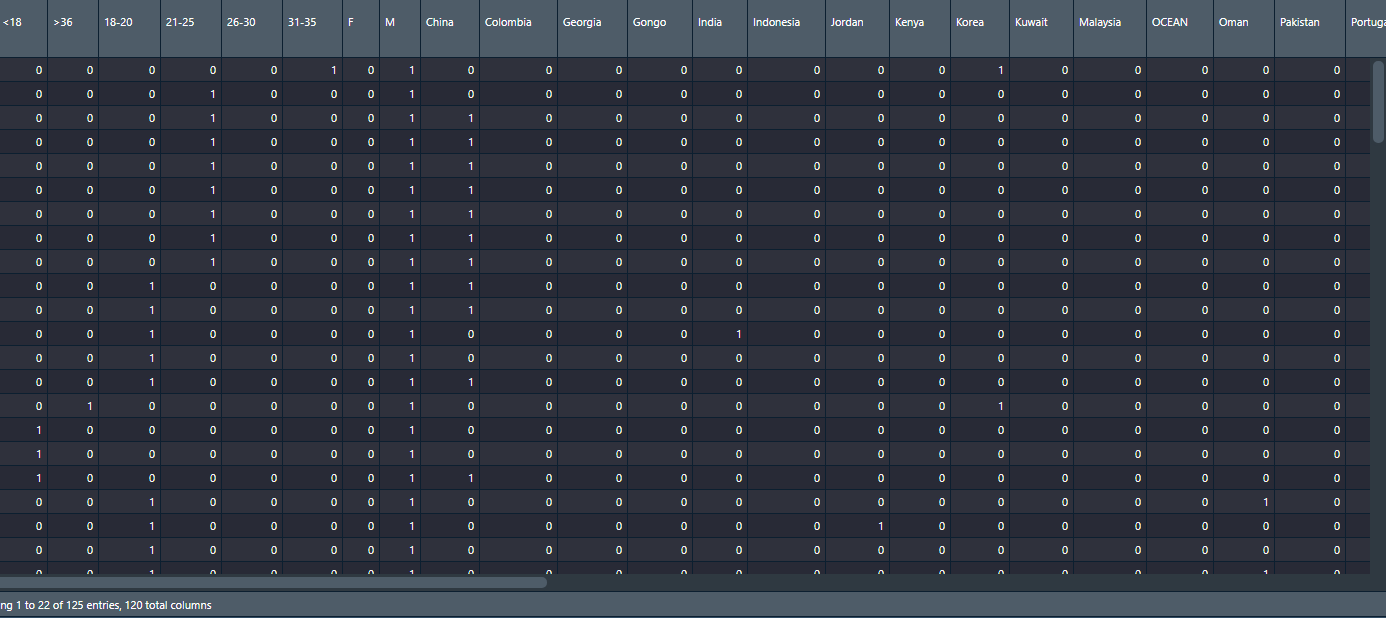
\includegraphics{tc.png}
\caption{tableau disjonctif complet}
\end{figure}

On a 125 individus, ici nous allons considérer que les modalités avec un
effectif moins de 5 sont trés faible, donc on va éliminer ces modalités,
nous avons opter pour cette option pour alléger un peu le nombre de
colonne {[} on avait 120 modalités{]}

\begin{Shaded}
\begin{Highlighting}[]
\NormalTok{n }\OtherTok{\textless{}{-}} \FunctionTok{nrow}\NormalTok{(df)}

\NormalTok{i }\OtherTok{\textless{}{-}} \DecValTok{1}

\ControlFlowTok{while}\NormalTok{( i }\SpecialCharTok{\textless{}=} \FunctionTok{ncol}\NormalTok{(df) )\{}

\NormalTok{  ns }\OtherTok{\textless{}{-}} \FunctionTok{sum}\NormalTok{(df[,i])}


  \ControlFlowTok{if}\NormalTok{( ns }\SpecialCharTok{\textless{}} \DecValTok{5}\NormalTok{  )\{}
\NormalTok{    df[,i] }\OtherTok{\textless{}{-}} \ConstantTok{NULL}
\NormalTok{    i }\OtherTok{\textless{}{-}} \DecValTok{1}
\NormalTok{  \}}

\NormalTok{  i }\OtherTok{\textless{}{-}}\NormalTok{ i }\SpecialCharTok{+} \DecValTok{1}
\NormalTok{\}}

\FunctionTok{print}\NormalTok{(}\FunctionTok{ncol}\NormalTok{(df))}
\end{Highlighting}
\end{Shaded}

\begin{verbatim}
## [1] 83
\end{verbatim}

\hypertarget{afcm-sur-le-questionnaire}{%
\section{AFCM sur le questionnaire :}\label{afcm-sur-le-questionnaire}}

Maintenant on a que 50 modalités , on va effectuer une AFC sur le
tableau disjonctif complet :

\begin{Shaded}
\begin{Highlighting}[]
\NormalTok{acm }\OtherTok{\textless{}{-}} \FunctionTok{CA}\NormalTok{(df,}\AttributeTok{graph =}\NormalTok{ F)}
\end{Highlighting}
\end{Shaded}

\hypertarget{valeurs-propres}{%
\subsection{valeurs propres :}\label{valeurs-propres}}

\begin{Shaded}
\begin{Highlighting}[]
\FunctionTok{barplot}\NormalTok{(acm}\SpecialCharTok{$}\NormalTok{eig[,}\DecValTok{1}\NormalTok{],acm}\SpecialCharTok{$}\NormalTok{eig[,}\DecValTok{2}\NormalTok{])}
\end{Highlighting}
\end{Shaded}

\includegraphics[width=1\linewidth]{AFCM_files/figure-latex/unnamed-chunk-35-1}
On remarque que pour avoir un pourcentage d'interie d'au moins 80\% il
faut prendre les 31 premiers axes factoriels :

\begin{Shaded}
\begin{Highlighting}[]
\NormalTok{acm}\SpecialCharTok{$}\NormalTok{eig[,}\DecValTok{3}\NormalTok{]}
\end{Highlighting}
\end{Shaded}

\begin{verbatim}
##      dim 1      dim 2      dim 3      dim 4      dim 5      dim 6      dim 7 
##   5.829481  11.165566  15.917393  20.304632  24.347954  27.713406  30.893056 
##      dim 8      dim 9     dim 10     dim 11     dim 12     dim 13     dim 14 
##  33.919162  36.899582  39.679400  42.365337  44.994096  47.559384  50.045942 
##     dim 15     dim 16     dim 17     dim 18     dim 19     dim 20     dim 21 
##  52.396586  54.702764  56.861417  58.892092  60.906383  62.871171  64.707398 
##     dim 22     dim 23     dim 24     dim 25     dim 26     dim 27     dim 28 
##  66.539137  68.353759  70.066838  71.708648  73.300710  74.795141  76.273933 
##     dim 29     dim 30     dim 31     dim 32     dim 33     dim 34     dim 35 
##  77.649512  79.009750  80.300424  81.541513  82.697804  83.827639  84.863634 
##     dim 36     dim 37     dim 38     dim 39     dim 40     dim 41     dim 42 
##  85.881294  86.867772  87.811578  88.698195  89.561735  90.413777  91.172662 
##     dim 43     dim 44     dim 45     dim 46     dim 47     dim 48     dim 49 
##  91.874625  92.543737  93.173313  93.773420  94.353767  94.846563  95.333173 
##     dim 50     dim 51     dim 52     dim 53     dim 54     dim 55     dim 56 
##  95.805537  96.267783  96.688434  97.073552  97.434829  97.768433  98.098014 
##     dim 57     dim 58     dim 59     dim 60     dim 61     dim 62     dim 63 
##  98.409787  98.672418  98.928277  99.165197  99.387126  99.588315  99.758696 
##     dim 64     dim 65     dim 66     dim 67     dim 68     dim 69     dim 70 
##  99.845942  99.891737  99.920066  99.942847  99.962533  99.975339  99.985640 
##     dim 71     dim 72     dim 73     dim 74     dim 75     dim 76     dim 77 
##  99.992352  99.997061 100.000000 100.000000 100.000000 100.000000 100.000000 
##     dim 78     dim 79     dim 80     dim 81     dim 82 
## 100.000000 100.000000 100.000000 100.000000 100.000000
\end{verbatim}

\hypertarget{le-biplot-individus-variables}{%
\subsection{le biplot individus-variables
:}\label{le-biplot-individus-variables}}

\begin{Shaded}
\begin{Highlighting}[]
\FunctionTok{plot.CA}\NormalTok{(acm)}
\end{Highlighting}
\end{Shaded}

\includegraphics[width=1\linewidth]{AFCM_files/figure-latex/unnamed-chunk-37-1}

\hypertarget{etude-du-tableau-des-contributions}{%
\subsection{Etude du tableau des
contributions:}\label{etude-du-tableau-des-contributions}}

Une variable contribue bien à la construction du premier axe si sa
contribution absolue est supérieue à son poids :

\begin{Shaded}
\begin{Highlighting}[]
\NormalTok{contribCol }\OtherTok{\textless{}{-}} \FunctionTok{as.data.frame}\NormalTok{(acm}\SpecialCharTok{$}\NormalTok{col}\SpecialCharTok{$}\NormalTok{contrib)}
\NormalTok{coordCol }\OtherTok{\textless{}{-}} \FunctionTok{as.data.frame}\NormalTok{(acm}\SpecialCharTok{$}\NormalTok{col}\SpecialCharTok{$}\NormalTok{coord)}

\NormalTok{contribRow }\OtherTok{\textless{}{-}} \FunctionTok{as.data.frame}\NormalTok{(acm}\SpecialCharTok{$}\NormalTok{row}\SpecialCharTok{$}\NormalTok{contrib)}
\NormalTok{coordRow }\OtherTok{\textless{}{-}} \FunctionTok{as.data.frame}\NormalTok{(acm}\SpecialCharTok{$}\NormalTok{row}\SpecialCharTok{$}\NormalTok{coord)}

\FunctionTok{print}\NormalTok{(}\StringTok{"\#\#\#\#\#\#\#\#\# Les variables qui contribuent le plus à la construction du premier axe \#\#\#\#\#\#\#\#\# "}\NormalTok{)}
\end{Highlighting}
\end{Shaded}

\begin{verbatim}
## [1] "######### Les variables qui contribuent le plus à la construction du premier axe ######### "
\end{verbatim}

\begin{Shaded}
\begin{Highlighting}[]
\ControlFlowTok{for}\NormalTok{(i }\ControlFlowTok{in} \DecValTok{1}\SpecialCharTok{:}\FunctionTok{ncol}\NormalTok{(df))\{}
  
\NormalTok{      ns }\OtherTok{\textless{}{-}} \FunctionTok{sum}\NormalTok{(df[,i])}
\NormalTok{      fs }\OtherTok{\textless{}{-}}\NormalTok{ ns }\SpecialCharTok{/}\NormalTok{n}
      
      \ControlFlowTok{if}\NormalTok{(contribCol}\SpecialCharTok{$}\StringTok{\textasciigrave{}}\AttributeTok{Dim 1}\StringTok{\textasciigrave{}}\NormalTok{[i] }\SpecialCharTok{\textgreater{}=}\NormalTok{ fs}\SpecialCharTok{*}\DecValTok{100} \SpecialCharTok{\&\&}\NormalTok{ coordCol}\SpecialCharTok{$}\StringTok{\textasciigrave{}}\AttributeTok{Dim 1}\StringTok{\textasciigrave{}}\NormalTok{[i] }\SpecialCharTok{\textgreater{}} \DecValTok{0}\NormalTok{)\{}
        \FunctionTok{print}\NormalTok{(}\FunctionTok{c}\NormalTok{(}\FunctionTok{colnames}\NormalTok{(df)[i],}\StringTok{"+"}\NormalTok{))}
\NormalTok{      \}}
      \ControlFlowTok{if}\NormalTok{(contribCol}\SpecialCharTok{$}\StringTok{\textasciigrave{}}\AttributeTok{Dim 1}\StringTok{\textasciigrave{}}\NormalTok{[i] }\SpecialCharTok{\textgreater{}=}\NormalTok{ fs}\SpecialCharTok{*}\DecValTok{100} \SpecialCharTok{\&\&}\NormalTok{ coordCol}\SpecialCharTok{$}\StringTok{\textasciigrave{}}\AttributeTok{Dim 1}\StringTok{\textasciigrave{}}\NormalTok{[i] }\SpecialCharTok{\textless{}} \DecValTok{0}\NormalTok{)\{}
        \FunctionTok{print}\NormalTok{(}\FunctionTok{c}\NormalTok{(}\FunctionTok{colnames}\NormalTok{(df)[i],}\StringTok{"{-}"}\NormalTok{))}
\NormalTok{      \}}
\NormalTok{\}}
\end{Highlighting}
\end{Shaded}

\begin{verbatim}
## [1] "X6_Strong Agree" "+"
\end{verbatim}

\begin{Shaded}
\begin{Highlighting}[]
\FunctionTok{print}\NormalTok{(}\StringTok{"\#\#\#\#\#\#\#\#\# Les individus qui contribuent le plus à la construction du premier axe \#\#\#\#\#\#\#\#\# "}\NormalTok{)}
\end{Highlighting}
\end{Shaded}

\begin{verbatim}
## [1] "######### Les individus qui contribuent le plus à la construction du premier axe ######### "
\end{verbatim}

\begin{Shaded}
\begin{Highlighting}[]
\ControlFlowTok{for}\NormalTok{(i }\ControlFlowTok{in} \DecValTok{1}\SpecialCharTok{:}\FunctionTok{nrow}\NormalTok{(df))\{}

      
      \ControlFlowTok{if}\NormalTok{(contribRow}\SpecialCharTok{$}\StringTok{\textasciigrave{}}\AttributeTok{Dim 1}\StringTok{\textasciigrave{}}\NormalTok{[i] }\SpecialCharTok{\textgreater{}} \DecValTok{100}\SpecialCharTok{/}\NormalTok{n }\SpecialCharTok{\&\&}\NormalTok{ coordRow}\SpecialCharTok{$}\StringTok{\textasciigrave{}}\AttributeTok{Dim 1}\StringTok{\textasciigrave{}}\NormalTok{[i] }\SpecialCharTok{\textgreater{}} \DecValTok{0}\NormalTok{)\{}
        \FunctionTok{print}\NormalTok{(}\FunctionTok{c}\NormalTok{(i,}\StringTok{"+"}\NormalTok{))}
\NormalTok{      \}}
      \ControlFlowTok{if}\NormalTok{(contribRow}\SpecialCharTok{$}\StringTok{\textasciigrave{}}\AttributeTok{Dim 1}\StringTok{\textasciigrave{}}\NormalTok{[i] }\SpecialCharTok{\textgreater{}} \DecValTok{100}\SpecialCharTok{/}\NormalTok{n }\SpecialCharTok{\&\&}\NormalTok{ coordRow}\SpecialCharTok{$}\StringTok{\textasciigrave{}}\AttributeTok{Dim 1}\StringTok{\textasciigrave{}}\NormalTok{[i] }\SpecialCharTok{\textless{}} \DecValTok{0}\NormalTok{)\{}
        \FunctionTok{print}\NormalTok{(}\FunctionTok{c}\NormalTok{(i,}\StringTok{"{-}"}\NormalTok{))}
\NormalTok{      \}}
\NormalTok{\}}
\end{Highlighting}
\end{Shaded}

\begin{verbatim}
## [1] "4" "-"
## [1] "7" "-"
## [1] "16" "+" 
## [1] "20" "+" 
## [1] "25" "+" 
## [1] "27" "+" 
## [1] "28" "+" 
## [1] "38" "-" 
## [1] "43" "+" 
## [1] "46" "-" 
## [1] "54" "+" 
## [1] "58" "-" 
## [1] "61" "-" 
## [1] "62" "-" 
## [1] "64" "-" 
## [1] "66" "-" 
## [1] "77" "+" 
## [1] "79" "+" 
## [1] "82" "+" 
## [1] "86" "+" 
## [1] "87" "+" 
## [1] "90" "+" 
## [1] "91" "-" 
## [1] "96" "-" 
## [1] "98" "-" 
## [1] "100" "-"  
## [1] "105" "-"  
## [1] "106" "-"  
## [1] "107" "-"  
## [1] "111" "-"  
## [1] "112" "+"  
## [1] "113" "+"  
## [1] "114" "-"  
## [1] "117" "-"  
## [1] "119" "-"  
## [1] "122" "+"
\end{verbatim}

\begin{Shaded}
\begin{Highlighting}[]
\FunctionTok{fviz\_contrib}\NormalTok{(acm, }\AttributeTok{choice =}\StringTok{"col"}\NormalTok{, }\AttributeTok{axes =} \DecValTok{1}\NormalTok{)}
\end{Highlighting}
\end{Shaded}

\includegraphics[width=1\linewidth]{AFCM_files/figure-latex/unnamed-chunk-38-1}

\begin{Shaded}
\begin{Highlighting}[]
\FunctionTok{fviz\_contrib}\NormalTok{(acm, }\AttributeTok{choice =}\StringTok{"row"}\NormalTok{, }\AttributeTok{axes =} \DecValTok{1}\NormalTok{)}
\end{Highlighting}
\end{Shaded}

\includegraphics[width=1\linewidth]{AFCM_files/figure-latex/unnamed-chunk-38-2}
On déduit que le premier axe est à effet taille, il caractèrise les
individus qui ont répondu à la question 6 avec '' tout à fait d'accord
``, représenté par les individus
16,20,25,27,28,43,54,77,79,82,86,87,90,112,113,122 contrairement aux
individus
4,7,38,46,58,61,62,64,66,91,96,98,100,105,106,107,111,114,117,119 qui
ont été en désaccord avec la question 6

\begin{Shaded}
\begin{Highlighting}[]
\FunctionTok{print}\NormalTok{(}\StringTok{"\#\#\#\#\#\#\#\#\# Les variables qui contribuent le plus à la construction du 2ème axe \#\#\#\#\#\#\#\#\# "}\NormalTok{)}
\end{Highlighting}
\end{Shaded}

\begin{verbatim}
## [1] "######### Les variables qui contribuent le plus à la construction du 2ème axe ######### "
\end{verbatim}

\begin{Shaded}
\begin{Highlighting}[]
\ControlFlowTok{for}\NormalTok{(i }\ControlFlowTok{in} \DecValTok{1}\SpecialCharTok{:}\FunctionTok{ncol}\NormalTok{(df))\{}
  
\NormalTok{      ns }\OtherTok{\textless{}{-}} \FunctionTok{sum}\NormalTok{(df[,i])}
\NormalTok{      fs }\OtherTok{\textless{}{-}}\NormalTok{ ns }\SpecialCharTok{/}\NormalTok{n}
      
      \ControlFlowTok{if}\NormalTok{(contribCol}\SpecialCharTok{$}\StringTok{\textasciigrave{}}\AttributeTok{Dim 2}\StringTok{\textasciigrave{}}\NormalTok{[i] }\SpecialCharTok{\textgreater{}}\NormalTok{ fs}\SpecialCharTok{*}\DecValTok{100} \SpecialCharTok{\&\&}\NormalTok{ coordCol}\SpecialCharTok{$}\StringTok{\textasciigrave{}}\AttributeTok{Dim 2}\StringTok{\textasciigrave{}}\NormalTok{[i] }\SpecialCharTok{\textgreater{}} \DecValTok{0}\NormalTok{)\{}
        \FunctionTok{print}\NormalTok{(}\FunctionTok{c}\NormalTok{(}\FunctionTok{colnames}\NormalTok{(df)[i],}\StringTok{"+"}\NormalTok{))}
\NormalTok{      \}}
      \ControlFlowTok{if}\NormalTok{(contribCol}\SpecialCharTok{$}\StringTok{\textasciigrave{}}\AttributeTok{Dim 2}\StringTok{\textasciigrave{}}\NormalTok{[i] }\SpecialCharTok{\textgreater{}}\NormalTok{ fs}\SpecialCharTok{*}\DecValTok{100} \SpecialCharTok{\&\&}\NormalTok{ coordCol}\SpecialCharTok{$}\StringTok{\textasciigrave{}}\AttributeTok{Dim 2}\StringTok{\textasciigrave{}}\NormalTok{[i] }\SpecialCharTok{\textless{}} \DecValTok{0}\NormalTok{)\{}
        \FunctionTok{print}\NormalTok{(}\FunctionTok{c}\NormalTok{(}\FunctionTok{colnames}\NormalTok{(df)[i],}\StringTok{"{-}"}\NormalTok{))}
\NormalTok{      \}}
      
\NormalTok{\}}
\end{Highlighting}
\end{Shaded}

\begin{verbatim}
## [1] "31-35" "+"
\end{verbatim}

\begin{Shaded}
\begin{Highlighting}[]
\FunctionTok{print}\NormalTok{(}\StringTok{"\#\#\#\#\#\#\#\#\# Les individus qui contribuent le plus à la construction du 2ème axe \#\#\#\#\#\#\#\#\# "}\NormalTok{)}
\end{Highlighting}
\end{Shaded}

\begin{verbatim}
## [1] "######### Les individus qui contribuent le plus à la construction du 2ème axe ######### "
\end{verbatim}

\begin{Shaded}
\begin{Highlighting}[]
\ControlFlowTok{for}\NormalTok{(i }\ControlFlowTok{in} \DecValTok{1}\SpecialCharTok{:}\FunctionTok{nrow}\NormalTok{(df))\{}
  
      
      \ControlFlowTok{if}\NormalTok{(contribRow}\SpecialCharTok{$}\StringTok{\textasciigrave{}}\AttributeTok{Dim 2}\StringTok{\textasciigrave{}}\NormalTok{[i] }\SpecialCharTok{\textgreater{}} \DecValTok{100}\SpecialCharTok{/}\NormalTok{n }\SpecialCharTok{\&\&}\NormalTok{ coordRow}\SpecialCharTok{$}\StringTok{\textasciigrave{}}\AttributeTok{Dim 2}\StringTok{\textasciigrave{}}\NormalTok{[i] }\SpecialCharTok{\textgreater{}} \DecValTok{0}\NormalTok{)\{}
        \FunctionTok{print}\NormalTok{(}\FunctionTok{c}\NormalTok{(i,}\StringTok{"+"}\NormalTok{))}
\NormalTok{      \}}
      \ControlFlowTok{if}\NormalTok{(contribRow}\SpecialCharTok{$}\StringTok{\textasciigrave{}}\AttributeTok{Dim 2}\StringTok{\textasciigrave{}}\NormalTok{[i] }\SpecialCharTok{\textgreater{}} \DecValTok{100}\SpecialCharTok{/}\NormalTok{n }\SpecialCharTok{\&\&}\NormalTok{ coordRow}\SpecialCharTok{$}\StringTok{\textasciigrave{}}\AttributeTok{Dim 2}\StringTok{\textasciigrave{}}\NormalTok{[i] }\SpecialCharTok{\textless{}} \DecValTok{0}\NormalTok{)\{}
        \FunctionTok{print}\NormalTok{(}\FunctionTok{c}\NormalTok{(i,}\StringTok{"{-}"}\NormalTok{))}
\NormalTok{      \}}
\NormalTok{\}}
\end{Highlighting}
\end{Shaded}

\begin{verbatim}
## [1] "1" "+"
## [1] "3" "+"
## [1] "5" "-"
## [1] "6" "+"
## [1] "11" "-" 
## [1] "16" "+" 
## [1] "20" "+" 
## [1] "26" "-" 
## [1] "27" "-" 
## [1] "28" "+" 
## [1] "30" "-" 
## [1] "31" "+" 
## [1] "36" "+" 
## [1] "43" "+" 
## [1] "45" "-" 
## [1] "49" "-" 
## [1] "59" "+" 
## [1] "69" "+" 
## [1] "73" "-" 
## [1] "76" "-" 
## [1] "80" "-" 
## [1] "82" "-" 
## [1] "88" "-" 
## [1] "89" "-" 
## [1] "98" "+" 
## [1] "101" "+"  
## [1] "112" "+"  
## [1] "113" "-"  
## [1] "118" "+"  
## [1] "120" "-"  
## [1] "122" "+"  
## [1] "125" "+"
\end{verbatim}

\begin{Shaded}
\begin{Highlighting}[]
\FunctionTok{fviz\_contrib}\NormalTok{(acm, }\AttributeTok{choice =}\StringTok{"col"}\NormalTok{, }\AttributeTok{axes =} \DecValTok{2}\NormalTok{)}
\end{Highlighting}
\end{Shaded}

\includegraphics[width=1\linewidth]{AFCM_files/figure-latex/unnamed-chunk-39-1}

\begin{Shaded}
\begin{Highlighting}[]
\FunctionTok{fviz\_contrib}\NormalTok{(acm, }\AttributeTok{choice =}\StringTok{"row"}\NormalTok{, }\AttributeTok{axes =} \DecValTok{2}\NormalTok{)}
\end{Highlighting}
\end{Shaded}

\includegraphics[width=1\linewidth]{AFCM_files/figure-latex/unnamed-chunk-39-2}
On déduit que le 2ème axe est à effet taille, il caractèrise les
étudiants qui ont déclaré que leurs age est compris entre 31 ans et 35
représenté par les individus
1,3,6,16,20,28,31,36,43,59,69,98,101,112,118,122,125 contrairement aux
individus 5,11,26,27,30,49,73,76,80,82,88,89,113,120

On remarque que certaines individus n'ont pas un age entre 31 et 35 mais
ils representent cet axe, on conclut donc que ces individus sont mal
représentés. Or on remarque aussi que ce premier plan factoriel ne
représente que 11.16\% de l'information contenue dans notre jeu de
données.

\hypertarget{les-fortes-association-quon-peut-ressortir-de-lafcm}{%
\subsection{Les fortes association qu'on peut ressortir de l'AFCM
:}\label{les-fortes-association-quon-peut-ressortir-de-lafcm}}

Ceux qui ont un age compris entre 31 et 35 ont tendance à étre tout à
fait d'accord avec la question 7

\begin{Shaded}
\begin{Highlighting}[]
\CommentTok{\# for (i in 1:ncol(df))\{}
\CommentTok{\#   for(j in 1:ncol(df))\{}
\CommentTok{\#     }
\CommentTok{\#     }
\CommentTok{\#     if( sqrt( ( coordCol$\textasciigrave{}Dim 1\textasciigrave{}[i] {-} coordCol$\textasciigrave{}Dim 1\textasciigrave{}[j] )**2 + ( coordCol$\textasciigrave{}Dim 2\textasciigrave{}[i] {-} coordCol$\textasciigrave{}Dim 2\textasciigrave{}[j] )**2 )  \textless{} 1 \&\& i != j)\{}
\CommentTok{\#       print(c(colnames(df)[i],colnames(df)[j]))}
\CommentTok{\#     \}}
\CommentTok{\#   \}}
\CommentTok{\# \# \}}
\CommentTok{\# fviz\_mca\_biplot(acm ,repel = TRUE)}
\end{Highlighting}
\end{Shaded}

\hypertarget{les-questions-les-mieux-repruxe9sentuxe9es-par-lafcm}{%
\subsection{Les questions les mieux représentées par l'AFCM
:}\label{les-questions-les-mieux-repruxe9sentuxe9es-par-lafcm}}

\begin{Shaded}
\begin{Highlighting}[]
\NormalTok{cosCol }\OtherTok{\textless{}{-}} \FunctionTok{as.data.frame}\NormalTok{(acm}\SpecialCharTok{$}\NormalTok{col}\SpecialCharTok{$}\NormalTok{cos2)}

\FunctionTok{print}\NormalTok{(}\StringTok{"\#\#\#\#\#\#\#\#\# Les variables les mieux représentées par le  premier axe \#\#\#\#\#\#\#\#\# "}\NormalTok{)}
\end{Highlighting}
\end{Shaded}

\begin{verbatim}
## [1] "######### Les variables les mieux représentées par le  premier axe ######### "
\end{verbatim}

\begin{Shaded}
\begin{Highlighting}[]
\ControlFlowTok{for}\NormalTok{(i }\ControlFlowTok{in} \DecValTok{1}\SpecialCharTok{:}\FunctionTok{ncol}\NormalTok{(df))\{}
  
      
      \ControlFlowTok{if}\NormalTok{(cosCol}\SpecialCharTok{$}\StringTok{\textasciigrave{}}\AttributeTok{Dim 1}\StringTok{\textasciigrave{}}\NormalTok{[i] }\SpecialCharTok{\textgreater{}=} \FloatTok{0.2}\NormalTok{ )\{}
        \FunctionTok{print}\NormalTok{(}\FunctionTok{colnames}\NormalTok{(df)[i])}
\NormalTok{      \}}
\NormalTok{\}}
\end{Highlighting}
\end{Shaded}

\begin{verbatim}
## [1] "21-25"
## [1] "IYO"
## [1] "PM"
## [1] "X6_Disagree"
## [1] "X6_Strong Agree"
## [1] "X16_Strong Agree"
## [1] "X17_Strong Disagree"
\end{verbatim}

\begin{Shaded}
\begin{Highlighting}[]
\FunctionTok{print}\NormalTok{(}\StringTok{"\#\#\#\#\#\#\#\#\# Les variables les mieux représentées par le 2ème axe \#\#\#\#\#\#\#\#\# "}\NormalTok{)}
\end{Highlighting}
\end{Shaded}

\begin{verbatim}
## [1] "######### Les variables les mieux représentées par le 2ème axe ######### "
\end{verbatim}

\begin{Shaded}
\begin{Highlighting}[]
\ControlFlowTok{for}\NormalTok{(i }\ControlFlowTok{in} \DecValTok{1}\SpecialCharTok{:}\FunctionTok{ncol}\NormalTok{(df))\{}
  
      
      \ControlFlowTok{if}\NormalTok{(cosCol}\SpecialCharTok{$}\StringTok{\textasciigrave{}}\AttributeTok{Dim 2}\StringTok{\textasciigrave{}}\NormalTok{[i] }\SpecialCharTok{\textgreater{}=} \FloatTok{0.2}\NormalTok{ )\{}
        \FunctionTok{print}\NormalTok{(}\FunctionTok{colnames}\NormalTok{(df)[i])}
\NormalTok{      \}}
\NormalTok{\}}
\end{Highlighting}
\end{Shaded}

\begin{verbatim}
## [1] "X6_Neither"
## [1] "X8_Neither"
## [1] "X12_Neither"
## [1] "X13_Neither"
\end{verbatim}

\hypertarget{afc-sur-deux-questions}{%
\section{AFC sur deux questions :}\label{afc-sur-deux-questions}}

\hypertarget{croiser-2-questions}{%
\subsection{Croiser 2 questions :}\label{croiser-2-questions}}

Ici nous cherchons à faire une AFC entre les 2 questions les plus
pertinentes, donc nous allons faire une recherche exaustive pour les
détécter

\begin{Shaded}
\begin{Highlighting}[]
\NormalTok{col1 }\OtherTok{\textless{}{-}} \SpecialCharTok{{-}}\DecValTok{1}
\NormalTok{col2 }\OtherTok{\textless{}{-}} \SpecialCharTok{{-}}\DecValTok{1}
\NormalTok{tc\_afc }\OtherTok{\textless{}{-}} \ConstantTok{NULL}
\NormalTok{p\_value }\OtherTok{\textless{}{-}} \DecValTok{1}

\ControlFlowTok{for}\NormalTok{( i }\ControlFlowTok{in} \DecValTok{1}\SpecialCharTok{:}\FunctionTok{ncol}\NormalTok{(data))\{}
  \ControlFlowTok{for}\NormalTok{(j }\ControlFlowTok{in} \DecValTok{1}\SpecialCharTok{:}\FunctionTok{ncol}\NormalTok{(data))\{}
    \ControlFlowTok{if}\NormalTok{( i }\SpecialCharTok{!=}\NormalTok{ j)\{}
\NormalTok{      tc }\OtherTok{\textless{}{-}} \FunctionTok{table}\NormalTok{(data[,i],data[,j])}
\NormalTok{      a }\OtherTok{\textless{}{-}} \FunctionTok{chisq.test}\NormalTok{(tc)}
      
      \ControlFlowTok{if}\NormalTok{( a}\SpecialCharTok{$}\NormalTok{p.value }\SpecialCharTok{\textless{}}\NormalTok{ p\_value)\{}
\NormalTok{        p\_value }\OtherTok{\textless{}{-}}\NormalTok{ a}\SpecialCharTok{$}\NormalTok{p.value}
\NormalTok{        col1 }\OtherTok{\textless{}{-}}\NormalTok{ i}
\NormalTok{        col2 }\OtherTok{\textless{}{-}}\NormalTok{ j}
\NormalTok{        tc\_afc }\OtherTok{\textless{}{-}}\NormalTok{ tc}
\NormalTok{      \}}
\NormalTok{    \}}
\NormalTok{  \}}
\NormalTok{\}}

\FunctionTok{print}\NormalTok{(}\FunctionTok{colnames}\NormalTok{(data)[col1])}
\end{Highlighting}
\end{Shaded}

\begin{verbatim}
## [1] "Age"
\end{verbatim}

\begin{Shaded}
\begin{Highlighting}[]
\FunctionTok{print}\NormalTok{(}\FunctionTok{colnames}\NormalTok{(data)[col2])}
\end{Highlighting}
\end{Shaded}

\begin{verbatim}
## [1] "Program"
\end{verbatim}

\begin{Shaded}
\begin{Highlighting}[]
\FunctionTok{print}\NormalTok{(p\_value)}
\end{Highlighting}
\end{Shaded}

\begin{verbatim}
## [1] 4.024138e-19
\end{verbatim}

\begin{Shaded}
\begin{Highlighting}[]
\NormalTok{tc\_afc}
\end{Highlighting}
\end{Shaded}

\begin{verbatim}
##        
##         FC IYO Language PM
##   <18    5   1        0  0
##   >36    1   1        1  1
##   18-20 21  12        0  3
##   21-25  4   1        0 57
##   26-30  0   0        0 12
##   31-35  0   0        0  5
\end{verbatim}

Donc on choisit la variable age et program

\begin{Shaded}
\begin{Highlighting}[]
\NormalTok{afc }\OtherTok{\textless{}{-}} \FunctionTok{CA}\NormalTok{(tc\_afc)}
\end{Highlighting}
\end{Shaded}

\includegraphics[width=1\linewidth]{AFCM_files/figure-latex/unnamed-chunk-43-1}

\hypertarget{valeurs-propres-1}{%
\subsection{valeurs propres :}\label{valeurs-propres-1}}

On remarque qu'avec seulement les 2 premiers axe on a une tres bonne
représentation

\begin{Shaded}
\begin{Highlighting}[]
\FunctionTok{barplot}\NormalTok{(afc}\SpecialCharTok{$}\NormalTok{eig[,}\DecValTok{1}\NormalTok{],afc}\SpecialCharTok{$}\NormalTok{eig[,}\DecValTok{2}\NormalTok{])}
\end{Highlighting}
\end{Shaded}

\includegraphics[width=1\linewidth]{AFCM_files/figure-latex/unnamed-chunk-44-1}

\hypertarget{etude-du-tableau-des-contributions-1}{%
\subsection{Etude du tableau des
contributions:}\label{etude-du-tableau-des-contributions-1}}

\begin{Shaded}
\begin{Highlighting}[]
\NormalTok{contribCol }\OtherTok{\textless{}{-}} \FunctionTok{as.data.frame}\NormalTok{(afc}\SpecialCharTok{$}\NormalTok{col}\SpecialCharTok{$}\NormalTok{contrib)}
\NormalTok{coordCol }\OtherTok{\textless{}{-}} \FunctionTok{as.data.frame}\NormalTok{(afc}\SpecialCharTok{$}\NormalTok{col}\SpecialCharTok{$}\NormalTok{coord)}

\NormalTok{contribRow }\OtherTok{\textless{}{-}} \FunctionTok{as.data.frame}\NormalTok{(afc}\SpecialCharTok{$}\NormalTok{row}\SpecialCharTok{$}\NormalTok{contrib)}
\NormalTok{coordRow }\OtherTok{\textless{}{-}} \FunctionTok{as.data.frame}\NormalTok{(afc}\SpecialCharTok{$}\NormalTok{row}\SpecialCharTok{$}\NormalTok{coord)}

\FunctionTok{print}\NormalTok{(}\StringTok{"\#\#\#\#\#\#\#\#\# Les profile colonnes qui contribuent le plus à la construction du premier axe \#\#\#\#\#\#\#\#\# "}\NormalTok{)}
\end{Highlighting}
\end{Shaded}

\begin{verbatim}
## [1] "######### Les profile colonnes qui contribuent le plus à la construction du premier axe ######### "
\end{verbatim}

\begin{Shaded}
\begin{Highlighting}[]
\ControlFlowTok{for}\NormalTok{(i }\ControlFlowTok{in} \DecValTok{1}\SpecialCharTok{:}\FunctionTok{ncol}\NormalTok{(tc\_afc))\{}
  
\NormalTok{      ns }\OtherTok{\textless{}{-}} \FunctionTok{sum}\NormalTok{(tc\_afc[,i])}
\NormalTok{      fs }\OtherTok{\textless{}{-}}\NormalTok{ ns }\SpecialCharTok{/}\NormalTok{n}
      
      \ControlFlowTok{if}\NormalTok{(contribCol}\SpecialCharTok{$}\StringTok{\textasciigrave{}}\AttributeTok{Dim 1}\StringTok{\textasciigrave{}}\NormalTok{[i] }\SpecialCharTok{\textgreater{}=}\NormalTok{ fs}\SpecialCharTok{*}\DecValTok{100} \SpecialCharTok{\&\&}\NormalTok{ coordCol}\SpecialCharTok{$}\StringTok{\textasciigrave{}}\AttributeTok{Dim 1}\StringTok{\textasciigrave{}}\NormalTok{[i] }\SpecialCharTok{\textgreater{}} \DecValTok{0}\NormalTok{)\{}
        \FunctionTok{print}\NormalTok{(}\FunctionTok{c}\NormalTok{(}\FunctionTok{colnames}\NormalTok{(tc\_afc)[i],}\StringTok{"+"}\NormalTok{))}
\NormalTok{      \}}
      \ControlFlowTok{if}\NormalTok{(contribCol}\SpecialCharTok{$}\StringTok{\textasciigrave{}}\AttributeTok{Dim 1}\StringTok{\textasciigrave{}}\NormalTok{[i] }\SpecialCharTok{\textgreater{}=}\NormalTok{ fs}\SpecialCharTok{*}\DecValTok{100} \SpecialCharTok{\&\&}\NormalTok{ coordCol}\SpecialCharTok{$}\StringTok{\textasciigrave{}}\AttributeTok{Dim 1}\StringTok{\textasciigrave{}}\NormalTok{[i] }\SpecialCharTok{\textless{}} \DecValTok{0}\NormalTok{)\{}
        \FunctionTok{print}\NormalTok{(}\FunctionTok{c}\NormalTok{(}\FunctionTok{colnames}\NormalTok{(tc\_afc)[i],}\StringTok{"{-}"}\NormalTok{))}
\NormalTok{      \}}
\NormalTok{\}}
\end{Highlighting}
\end{Shaded}

\begin{verbatim}
## [1] "FC" "+" 
## [1] "IYO" "+"
\end{verbatim}

\begin{Shaded}
\begin{Highlighting}[]
\FunctionTok{print}\NormalTok{(}\StringTok{"\#\#\#\#\#\#\#\#\# Les profiles lignes qui contribuent le plus à la construction du premier axe \#\#\#\#\#\#\#\#\# "}\NormalTok{)}
\end{Highlighting}
\end{Shaded}

\begin{verbatim}
## [1] "######### Les profiles lignes qui contribuent le plus à la construction du premier axe ######### "
\end{verbatim}

\begin{Shaded}
\begin{Highlighting}[]
\ControlFlowTok{for}\NormalTok{(i }\ControlFlowTok{in} \DecValTok{1}\SpecialCharTok{:}\FunctionTok{nrow}\NormalTok{(tc\_afc))\{}
  
\NormalTok{      ns }\OtherTok{\textless{}{-}} \FunctionTok{sum}\NormalTok{(tc\_afc[i,])}
\NormalTok{      fs }\OtherTok{\textless{}{-}}\NormalTok{ ns }\SpecialCharTok{/}\NormalTok{n}

      \ControlFlowTok{if}\NormalTok{(contribRow}\SpecialCharTok{$}\StringTok{\textasciigrave{}}\AttributeTok{Dim 1}\StringTok{\textasciigrave{}}\NormalTok{[i] }\SpecialCharTok{\textgreater{}}\NormalTok{ fs}\SpecialCharTok{*}\DecValTok{100} \SpecialCharTok{\&\&}\NormalTok{ coordRow}\SpecialCharTok{$}\StringTok{\textasciigrave{}}\AttributeTok{Dim 1}\StringTok{\textasciigrave{}}\NormalTok{[i] }\SpecialCharTok{\textgreater{}} \DecValTok{0}\NormalTok{)\{}
        \FunctionTok{print}\NormalTok{(}\FunctionTok{c}\NormalTok{(}\FunctionTok{rownames}\NormalTok{(tc\_afc)[i],}\StringTok{"+"}\NormalTok{))}
\NormalTok{      \}}
      \ControlFlowTok{if}\NormalTok{(contribRow}\SpecialCharTok{$}\StringTok{\textasciigrave{}}\AttributeTok{Dim 1}\StringTok{\textasciigrave{}}\NormalTok{[i] }\SpecialCharTok{\textgreater{}}\NormalTok{ fs}\SpecialCharTok{*}\DecValTok{100} \SpecialCharTok{\&\&}\NormalTok{ coordRow}\SpecialCharTok{$}\StringTok{\textasciigrave{}}\AttributeTok{Dim 1}\StringTok{\textasciigrave{}}\NormalTok{[i] }\SpecialCharTok{\textless{}} \DecValTok{0}\NormalTok{)\{}
        \FunctionTok{print}\NormalTok{(}\FunctionTok{c}\NormalTok{(}\FunctionTok{rownames}\NormalTok{(tc\_afc)[i],}\StringTok{"{-}"}\NormalTok{))}
\NormalTok{      \}}
\NormalTok{\}}
\end{Highlighting}
\end{Shaded}

\begin{verbatim}
## [1] "<18" "+"  
## [1] "18-20" "+"
\end{verbatim}

On déduit que le premier axe est à effet taille, il quantifie les
classes qui ont beaucoup d'absences {[}s3{]} représenté par les
individus qui ont des moyennes comprises entre 49\% et 40\% dans les
cours académique et aussi les classes qui ont énormément d'absences
{[}s4{]} représenté par les individus qui ont des moyennes inférieure à
40\%.

\begin{Shaded}
\begin{Highlighting}[]
\FunctionTok{print}\NormalTok{(}\StringTok{"\#\#\#\#\#\#\#\#\# Les profile colonnes qui contribuent le plus à la construction du 2ème axe \#\#\#\#\#\#\#\#\# "}\NormalTok{)}
\end{Highlighting}
\end{Shaded}

\begin{verbatim}
## [1] "######### Les profile colonnes qui contribuent le plus à la construction du 2ème axe ######### "
\end{verbatim}

\begin{Shaded}
\begin{Highlighting}[]
\ControlFlowTok{for}\NormalTok{(i }\ControlFlowTok{in} \DecValTok{1}\SpecialCharTok{:}\FunctionTok{ncol}\NormalTok{(tc\_afc))\{}
  
\NormalTok{      ns }\OtherTok{\textless{}{-}} \FunctionTok{sum}\NormalTok{(tc\_afc[,i])}
\NormalTok{      fs }\OtherTok{\textless{}{-}}\NormalTok{ ns }\SpecialCharTok{/}\NormalTok{n}
      
      \ControlFlowTok{if}\NormalTok{(contribCol}\SpecialCharTok{$}\StringTok{\textasciigrave{}}\AttributeTok{Dim 2}\StringTok{\textasciigrave{}}\NormalTok{[i] }\SpecialCharTok{\textgreater{}=}\NormalTok{ fs}\SpecialCharTok{*}\DecValTok{100} \SpecialCharTok{\&\&}\NormalTok{ coordCol}\SpecialCharTok{$}\StringTok{\textasciigrave{}}\AttributeTok{Dim 2}\StringTok{\textasciigrave{}}\NormalTok{[i] }\SpecialCharTok{\textgreater{}} \DecValTok{0}\NormalTok{)\{}
        \FunctionTok{print}\NormalTok{(}\FunctionTok{c}\NormalTok{(}\FunctionTok{colnames}\NormalTok{(tc\_afc)[i],}\StringTok{"+"}\NormalTok{))}
\NormalTok{      \}}
      \ControlFlowTok{if}\NormalTok{(contribCol}\SpecialCharTok{$}\StringTok{\textasciigrave{}}\AttributeTok{Dim 2}\StringTok{\textasciigrave{}}\NormalTok{[i] }\SpecialCharTok{\textgreater{}=}\NormalTok{ fs}\SpecialCharTok{*}\DecValTok{100} \SpecialCharTok{\&\&}\NormalTok{ coordCol}\SpecialCharTok{$}\StringTok{\textasciigrave{}}\AttributeTok{Dim 2}\StringTok{\textasciigrave{}}\NormalTok{[i] }\SpecialCharTok{\textless{}} \DecValTok{0}\NormalTok{)\{}
        \FunctionTok{print}\NormalTok{(}\FunctionTok{c}\NormalTok{(}\FunctionTok{colnames}\NormalTok{(tc\_afc)[i],}\StringTok{"{-}"}\NormalTok{))}
\NormalTok{      \}}
\NormalTok{\}}
\end{Highlighting}
\end{Shaded}

\begin{verbatim}
## [1] "Language" "+"
\end{verbatim}

\begin{Shaded}
\begin{Highlighting}[]
\FunctionTok{print}\NormalTok{(}\StringTok{"\#\#\#\#\#\#\#\#\# Les profiles lignes qui contribuent le plus à la construction du 2ème axe \#\#\#\#\#\#\#\#\# "}\NormalTok{)}
\end{Highlighting}
\end{Shaded}

\begin{verbatim}
## [1] "######### Les profiles lignes qui contribuent le plus à la construction du 2ème axe ######### "
\end{verbatim}

\begin{Shaded}
\begin{Highlighting}[]
\ControlFlowTok{for}\NormalTok{(i }\ControlFlowTok{in} \DecValTok{1}\SpecialCharTok{:}\FunctionTok{nrow}\NormalTok{(tc\_afc))\{}
  
\NormalTok{      ns }\OtherTok{\textless{}{-}} \FunctionTok{sum}\NormalTok{(tc\_afc[i,])}
\NormalTok{      fs }\OtherTok{\textless{}{-}}\NormalTok{ ns }\SpecialCharTok{/}\NormalTok{n}

      \ControlFlowTok{if}\NormalTok{(contribRow}\SpecialCharTok{$}\StringTok{\textasciigrave{}}\AttributeTok{Dim 2}\StringTok{\textasciigrave{}}\NormalTok{[i] }\SpecialCharTok{\textgreater{}}\NormalTok{ fs}\SpecialCharTok{*}\DecValTok{100} \SpecialCharTok{\&\&}\NormalTok{ coordRow}\SpecialCharTok{$}\StringTok{\textasciigrave{}}\AttributeTok{Dim 2}\StringTok{\textasciigrave{}}\NormalTok{[i] }\SpecialCharTok{\textgreater{}} \DecValTok{0}\NormalTok{)\{}
        \FunctionTok{print}\NormalTok{(}\FunctionTok{c}\NormalTok{(}\FunctionTok{rownames}\NormalTok{(tc\_afc)[i],}\StringTok{"+"}\NormalTok{))}
\NormalTok{      \}}
      \ControlFlowTok{if}\NormalTok{(contribRow}\SpecialCharTok{$}\StringTok{\textasciigrave{}}\AttributeTok{Dim 2}\StringTok{\textasciigrave{}}\NormalTok{[i] }\SpecialCharTok{\textgreater{}}\NormalTok{ fs}\SpecialCharTok{*}\DecValTok{100} \SpecialCharTok{\&\&}\NormalTok{ coordRow}\SpecialCharTok{$}\StringTok{\textasciigrave{}}\AttributeTok{Dim 2}\StringTok{\textasciigrave{}}\NormalTok{[i] }\SpecialCharTok{\textless{}} \DecValTok{0}\NormalTok{)\{}
        \FunctionTok{print}\NormalTok{(}\FunctionTok{c}\NormalTok{(}\FunctionTok{rownames}\NormalTok{(tc\_afc)[i],}\StringTok{"{-}"}\NormalTok{))}
\NormalTok{      \}}
\NormalTok{\}}
\end{Highlighting}
\end{Shaded}

\begin{verbatim}
## [1] ">36" "+"
\end{verbatim}

Aussi le 2ème axe est à effet taille, il quantifie les classes qui ont
beaucoup beaucoup d'absences {[}s4{]} représenté par les individus qui
ont des moyenne inférieure à 40\% dans les cours académique.

\hypertarget{conclusion}{%
\section{Conclusion :}\label{conclusion}}

D'aprés les résultats obtenus on conclut que :

\begin{itemize}
\tightlist
\item
  Les étudiant qui s'absentent beaucoup ont tendance à avoir des
  moyennes faibles inférieure à 40\%
\end{itemize}

\end{document}
